\begin{tikzpicture}[scale=.2, anchor=base]
  \node[draw=black] (sn0x94e5990W9) at (9, -10) {\begin{tikzpicture}[scale=.2]
      \node[circle, scale=0.75, fill] (tid0) at (4.5,0){};
      \node[circle, scale=0.75, fill] (tid1) at (2.25,1.5){};
      \node[circle, scale=0.75, fill, red] (tid4) at (0.75,3){};
      \node[circle, scale=0.75, fill] (tid5) at (2.25,3){};
      \node[circle, scale=0.75, fill] (tid6) at (3.75,3){};
      \draw[](tid1) -- (tid4);
      \draw[](tid1) -- (tid5);
      \draw[](tid1) -- (tid6);
      \node[circle, scale=0.75, fill] (tid2) at (6,1.5){};
      \node[circle, scale=0.75, fill, red] (tid7) at (5.25,3){};
      \node[circle, scale=0.75, fill] (tid8) at (6.75,3){};
      \draw[](tid2) -- (tid7);
      \draw[](tid2) -- (tid8);
      \node[circle, scale=0.75, fill] (tid3) at (8.25,1.5){};
      \node[circle, scale=0.75, fill] (tid9) at (8.25,3){};
      \draw[](tid3) -- (tid9);
      \draw[](tid0) -- (tid1);
      \draw[](tid0) -- (tid2);
      \draw[](tid0) -- (tid3);

    \end{tikzpicture}
  };
  \node[draw=black] (sn0x94e5730W9) at (9, -20) {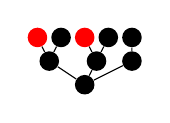
\begin{tikzpicture}[scale=.2]
      \node[circle, scale=0.75, fill] (tid0) at (3.75,0){};
      \node[circle, scale=0.75, fill] (tid1) at (1.5,1.5){};
      \node[circle, scale=0.75, fill, red] (tid4) at (0.75,3){};
      \node[circle, scale=0.75, fill] (tid5) at (2.25,3){};
      \draw[](tid1) -- (tid4);
      \draw[](tid1) -- (tid5);
      \node[circle, scale=0.75, fill] (tid2) at (4.5,1.5){};
      \node[circle, scale=0.75, fill, red] (tid6) at (3.75,3){};
      \node[circle, scale=0.75, fill] (tid7) at (5.25,3){};
      \draw[](tid2) -- (tid6);
      \draw[](tid2) -- (tid7);
      \node[circle, scale=0.75, fill] (tid3) at (6.75,1.5){};
      \node[circle, scale=0.75, fill] (tid8) at (6.75,3){};
      \draw[](tid3) -- (tid8);
      \draw[](tid0) -- (tid1);
      \draw[](tid0) -- (tid2);
      \draw[](tid0) -- (tid3);

    \end{tikzpicture}
  };
  \node[draw=black] (sn0x94e66c8W9) at (9, -30) {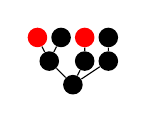
\begin{tikzpicture}[scale=.2]
      \node[circle, scale=0.75, fill] (tid0) at (3,0){};
      \node[circle, scale=0.75, fill] (tid1) at (1.5,1.5){};
      \node[circle, scale=0.75, fill, red] (tid4) at (0.75,3){};
      \node[circle, scale=0.75, fill] (tid5) at (2.25,3){};
      \draw[](tid1) -- (tid4);
      \draw[](tid1) -- (tid5);
      \node[circle, scale=0.75, fill] (tid2) at (3.75,1.5){};
      \node[circle, scale=0.75, fill, red] (tid6) at (3.75,3){};
      \draw[](tid2) -- (tid6);
      \node[circle, scale=0.75, fill] (tid3) at (5.25,1.5){};
      \node[circle, scale=0.75, fill] (tid7) at (5.25,3){};
      \draw[](tid3) -- (tid7);
      \draw[](tid0) -- (tid1);
      \draw[](tid0) -- (tid2);
      \draw[](tid0) -- (tid3);

    \end{tikzpicture}
  };
  \node[draw=black] (sn0x94e9fd8W9) at (9, -40) {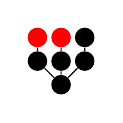
\begin{tikzpicture}[scale=.2]
      \node[circle, scale=0.75, fill] (tid0) at (2.25,0){};
      \node[circle, scale=0.75, fill] (tid1) at (0.75,1.5){};
      \node[circle, scale=0.75, fill, red] (tid4) at (0.75,3){};
      \draw[](tid1) -- (tid4);
      \node[circle, scale=0.75, fill] (tid2) at (2.25,1.5){};
      \node[circle, scale=0.75, fill, red] (tid5) at (2.25,3){};
      \draw[](tid2) -- (tid5);
      \node[circle, scale=0.75, fill] (tid3) at (3.75,1.5){};
      \node[circle, scale=0.75, fill] (tid6) at (3.75,3){};
      \draw[](tid3) -- (tid6);
      \draw[](tid0) -- (tid1);
      \draw[](tid0) -- (tid2);
      \draw[](tid0) -- (tid3);

    \end{tikzpicture}
  };
  \node[draw=black] (sn0x94ea750W9) at (9, -50) {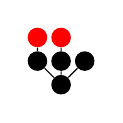
\begin{tikzpicture}[scale=.2]
      \node[circle, scale=0.75, fill] (tid0) at (2.25,0){};
      \node[circle, scale=0.75, fill] (tid1) at (0.75,1.5){};
      \node[circle, scale=0.75, fill, red] (tid4) at (0.75,3){};
      \draw[](tid1) -- (tid4);
      \node[circle, scale=0.75, fill] (tid2) at (2.25,1.5){};
      \node[circle, scale=0.75, fill, red] (tid5) at (2.25,3){};
      \draw[](tid2) -- (tid5);
      \node[circle, scale=0.75, fill] (tid3) at (3.75,1.5){};
      \draw[](tid0) -- (tid1);
      \draw[](tid0) -- (tid2);
      \draw[](tid0) -- (tid3);

    \end{tikzpicture}
  };
  \node[draw=black] (sn0x94eaa10W9) at (9, -60) {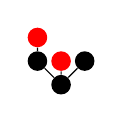
\begin{tikzpicture}[scale=.2]
      \node[circle, scale=0.75, fill] (tid0) at (2.25,0){};
      \node[circle, scale=0.75, fill] (tid1) at (0.75,1.5){};
      \node[circle, scale=0.75, fill, red] (tid4) at (0.75,3){};
      \draw[](tid1) -- (tid4);
      \node[circle, scale=0.75, fill, red] (tid2) at (2.25,1.5){};
      \node[circle, scale=0.75, fill] (tid3) at (3.75,1.5){};
      \draw[](tid0) -- (tid1);
      \draw[](tid0) -- (tid2);
      \draw[](tid0) -- (tid3);

    \end{tikzpicture}
  };
  \node[draw=black] (sn0x94ea990W9) at (9, -70) {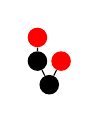
\begin{tikzpicture}[scale=.2]
      \node[circle, scale=0.75, fill] (tid0) at (1.5,0){};
      \node[circle, scale=0.75, fill] (tid1) at (0.75,1.5){};
      \node[circle, scale=0.75, fill, red] (tid3) at (0.75,3){};
      \draw[](tid1) -- (tid3);
      \node[circle, scale=0.75, fill, red] (tid2) at (2.25,1.5){};
      \draw[](tid0) -- (tid1);
      \draw[](tid0) -- (tid2);

    \end{tikzpicture}
  };
  \node[draw=black] (sn0x94ead40W9) at (9, -80) {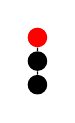
\begin{tikzpicture}[scale=.2]
      \node[circle, scale=0.75, fill] (tid0) at (0.75,0){};
      \node[circle, scale=0.75, fill] (tid1) at (0.75,1.5){};
      \node[circle, scale=0.75, fill, red] (tid2) at (0.75,3){};
      \draw[](tid1) -- (tid2);
      \draw[](tid0) -- (tid1);

    \end{tikzpicture}
  };
  \node[draw=black] (sn0x94eb148W9) at (9, -90) {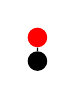
\begin{tikzpicture}[scale=.2]
      \node[circle, scale=0.75, fill] (tid0) at (0.75,0){};
      \node[circle, scale=0.75, fill, red] (tid1) at (0.75,1.5){};
      \draw[](tid0) -- (tid1);

    \end{tikzpicture}
  };
  \node[draw=black] (sn0x94eb1b0W9) at (9, -100) {
\begin{tikzpicture}[scale=.2]
      \node[circle, scale=0.75, fill, red] (tid0) at (0.75,0){};

    \end{tikzpicture}
  };
  \draw (sn0x94eb148W9.south) -- (sn0x94eb1b0W9.north);
  \draw (sn0x94ead40W9.south) -- (sn0x94eb148W9.north);
  \node[draw=black] (sn0x94eaff8W18) at (18, -80) {
\begin{tikzpicture}[scale=.2]
      \node[circle, scale=0.75, fill] (tid0) at (1.5,0){};
      \node[circle, scale=0.75, fill, red] (tid1) at (0.75,1.5){};
      \node[circle, scale=0.75, fill, red] (tid2) at (2.25,1.5){};
      \draw[](tid0) -- (tid1);
      \draw[](tid0) -- (tid2);

    \end{tikzpicture}
  };
  \draw (sn0x94eaff8W18.south) -- (sn0x94eb148W9.north);
  \draw (sn0x94ea990W9.south) -- (sn0x94ead40W9.north);
  \draw (sn0x94ea990W9.south) -- (sn0x94eaff8W18.north);
  \node[draw=black] (sn0x94eacd8W18) at (18, -70) {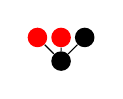
\begin{tikzpicture}[scale=.2]
      \node[circle, scale=0.75, fill] (tid0) at (2.25,0){};
      \node[circle, scale=0.75, fill, red] (tid1) at (0.75,1.5){};
      \node[circle, scale=0.75, fill, red] (tid2) at (2.25,1.5){};
      \node[circle, scale=0.75, fill] (tid3) at (3.75,1.5){};
      \draw[](tid0) -- (tid1);
      \draw[](tid0) -- (tid2);
      \draw[](tid0) -- (tid3);

    \end{tikzpicture}
  };
  \draw (sn0x94eacd8W18.south) -- (sn0x94eaff8W18.north);
  \draw (sn0x94eaa10W9.south) -- (sn0x94ea990W9.north);
  \draw (sn0x94eaa10W9.south) -- (sn0x94eacd8W18.north);
  \draw (sn0x94ea750W9.south) -- (sn0x94eaa10W9.north);
  \draw (sn0x94e9fd8W9.south) -- (sn0x94ea750W9.north);
  \node[draw=black] (sn0x94ea1a0W18) at (18, -40) {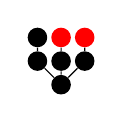
\begin{tikzpicture}[scale=.2]
      \node[circle, scale=0.75, fill] (tid0) at (2.25,0){};
      \node[circle, scale=0.75, fill] (tid1) at (0.75,1.5){};
      \node[circle, scale=0.75, fill] (tid4) at (0.75,3){};
      \draw[](tid1) -- (tid4);
      \node[circle, scale=0.75, fill] (tid2) at (2.25,1.5){};
      \node[circle, scale=0.75, fill, red] (tid5) at (2.25,3){};
      \draw[](tid2) -- (tid5);
      \node[circle, scale=0.75, fill] (tid3) at (3.75,1.5){};
      \node[circle, scale=0.75, fill, red] (tid6) at (3.75,3){};
      \draw[](tid3) -- (tid6);
      \draw[](tid0) -- (tid1);
      \draw[](tid0) -- (tid2);
      \draw[](tid0) -- (tid3);

    \end{tikzpicture}
  };
  \draw (sn0x94ea1a0W18.south) -- (sn0x94ea750W9.north);
  \node[draw=black] (sn0x94ea4b8W27) at (27, -40) {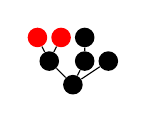
\begin{tikzpicture}[scale=.2]
      \node[circle, scale=0.75, fill] (tid0) at (3,0){};
      \node[circle, scale=0.75, fill] (tid1) at (1.5,1.5){};
      \node[circle, scale=0.75, fill, red] (tid4) at (0.75,3){};
      \node[circle, scale=0.75, fill, red] (tid5) at (2.25,3){};
      \draw[](tid1) -- (tid4);
      \draw[](tid1) -- (tid5);
      \node[circle, scale=0.75, fill] (tid2) at (3.75,1.5){};
      \node[circle, scale=0.75, fill] (tid6) at (3.75,3){};
      \draw[](tid2) -- (tid6);
      \node[circle, scale=0.75, fill] (tid3) at (5.25,1.5){};
      \draw[](tid0) -- (tid1);
      \draw[](tid0) -- (tid2);
      \draw[](tid0) -- (tid3);

    \end{tikzpicture}
  };
  \draw (sn0x94ea4b8W27.south) -- (sn0x94ea750W9.north);
  \node[draw=black] (sn0x94ea520W36) at (36, -40) {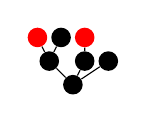
\begin{tikzpicture}[scale=.2]
      \node[circle, scale=0.75, fill] (tid0) at (3,0){};
      \node[circle, scale=0.75, fill] (tid1) at (1.5,1.5){};
      \node[circle, scale=0.75, fill, red] (tid4) at (0.75,3){};
      \node[circle, scale=0.75, fill] (tid5) at (2.25,3){};
      \draw[](tid1) -- (tid4);
      \draw[](tid1) -- (tid5);
      \node[circle, scale=0.75, fill] (tid2) at (3.75,1.5){};
      \node[circle, scale=0.75, fill, red] (tid6) at (3.75,3){};
      \draw[](tid2) -- (tid6);
      \node[circle, scale=0.75, fill] (tid3) at (5.25,1.5){};
      \draw[](tid0) -- (tid1);
      \draw[](tid0) -- (tid2);
      \draw[](tid0) -- (tid3);

    \end{tikzpicture}
  };
  \node[draw=black] (sn0x94eb378W18) at (18, -50) {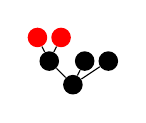
\begin{tikzpicture}[scale=.2]
      \node[circle, scale=0.75, fill] (tid0) at (3,0){};
      \node[circle, scale=0.75, fill] (tid1) at (1.5,1.5){};
      \node[circle, scale=0.75, fill, red] (tid4) at (0.75,3){};
      \node[circle, scale=0.75, fill, red] (tid5) at (2.25,3){};
      \draw[](tid1) -- (tid4);
      \draw[](tid1) -- (tid5);
      \node[circle, scale=0.75, fill] (tid2) at (3.75,1.5){};
      \node[circle, scale=0.75, fill] (tid3) at (5.25,1.5){};
      \draw[](tid0) -- (tid1);
      \draw[](tid0) -- (tid2);
      \draw[](tid0) -- (tid3);

    \end{tikzpicture}
  };
  \draw (sn0x94eb378W18.south) -- (sn0x94eaa10W9.north);
  \draw (sn0x94ea520W36.south) -- (sn0x94ea750W9.north);
  \draw (sn0x94ea520W36.south) -- (sn0x94eb378W18.north);
  \draw (sn0x94e66c8W9.south) -- (sn0x94e9fd8W9.north);
  \draw (sn0x94e66c8W9.south) -- (sn0x94ea1a0W18.north);
  \draw (sn0x94e66c8W9.south) -- (sn0x94ea4b8W27.north);
  \draw (sn0x94e66c8W9.south) -- (sn0x94ea520W36.north);
  \node[draw=black] (sn0x94e5588W18) at (18, -30) {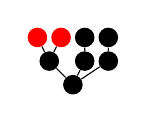
\begin{tikzpicture}[scale=.2]
      \node[circle, scale=0.75, fill] (tid0) at (3,0){};
      \node[circle, scale=0.75, fill] (tid1) at (1.5,1.5){};
      \node[circle, scale=0.75, fill, red] (tid4) at (0.75,3){};
      \node[circle, scale=0.75, fill, red] (tid5) at (2.25,3){};
      \draw[](tid1) -- (tid4);
      \draw[](tid1) -- (tid5);
      \node[circle, scale=0.75, fill] (tid2) at (3.75,1.5){};
      \node[circle, scale=0.75, fill] (tid6) at (3.75,3){};
      \draw[](tid2) -- (tid6);
      \node[circle, scale=0.75, fill] (tid3) at (5.25,1.5){};
      \node[circle, scale=0.75, fill] (tid7) at (5.25,3){};
      \draw[](tid3) -- (tid7);
      \draw[](tid0) -- (tid1);
      \draw[](tid0) -- (tid2);
      \draw[](tid0) -- (tid3);

    \end{tikzpicture}
  };
  \node[draw=black] (sn0x94ebd08W45) at (45, -40) {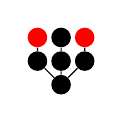
\begin{tikzpicture}[scale=.2]
      \node[circle, scale=0.75, fill] (tid0) at (2.25,0){};
      \node[circle, scale=0.75, fill] (tid1) at (0.75,1.5){};
      \node[circle, scale=0.75, fill, red] (tid4) at (0.75,3){};
      \draw[](tid1) -- (tid4);
      \node[circle, scale=0.75, fill] (tid2) at (2.25,1.5){};
      \node[circle, scale=0.75, fill] (tid5) at (2.25,3){};
      \draw[](tid2) -- (tid5);
      \node[circle, scale=0.75, fill] (tid3) at (3.75,1.5){};
      \node[circle, scale=0.75, fill, red] (tid6) at (3.75,3){};
      \draw[](tid3) -- (tid6);
      \draw[](tid0) -- (tid1);
      \draw[](tid0) -- (tid2);
      \draw[](tid0) -- (tid3);

    \end{tikzpicture}
  };
  \draw (sn0x94ebd08W45.south) -- (sn0x94ea750W9.north);
  \draw (sn0x94e5588W18.south) -- (sn0x94e9fd8W9.north);
  \draw (sn0x94e5588W18.south) -- (sn0x94ebd08W45.north);
  \node[draw=black] (sn0x94e6108W27) at (27, -30) {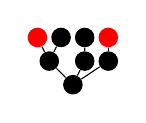
\begin{tikzpicture}[scale=.2]
      \node[circle, scale=0.75, fill] (tid0) at (3,0){};
      \node[circle, scale=0.75, fill] (tid1) at (1.5,1.5){};
      \node[circle, scale=0.75, fill, red] (tid4) at (0.75,3){};
      \node[circle, scale=0.75, fill] (tid5) at (2.25,3){};
      \draw[](tid1) -- (tid4);
      \draw[](tid1) -- (tid5);
      \node[circle, scale=0.75, fill] (tid2) at (3.75,1.5){};
      \node[circle, scale=0.75, fill] (tid6) at (3.75,3){};
      \draw[](tid2) -- (tid6);
      \node[circle, scale=0.75, fill] (tid3) at (5.25,1.5){};
      \node[circle, scale=0.75, fill, red] (tid7) at (5.25,3){};
      \draw[](tid3) -- (tid7);
      \draw[](tid0) -- (tid1);
      \draw[](tid0) -- (tid2);
      \draw[](tid0) -- (tid3);

    \end{tikzpicture}
  };
  \draw (sn0x94e6108W27.south) -- (sn0x94ebd08W45.north);
  \draw (sn0x94e6108W27.south) -- (sn0x94ea1a0W18.north);
  \draw (sn0x94e6108W27.south) -- (sn0x94ea4b8W27.north);
  \draw (sn0x94e6108W27.south) -- (sn0x94ea520W36.north);
  \draw (sn0x94e5730W9.south) -- (sn0x94e66c8W9.north);
  \draw (sn0x94e5730W9.south) -- (sn0x94e5588W18.north);
  \draw (sn0x94e5730W9.south) -- (sn0x94e6108W27.north);
  \node[draw=black] (sn0x94e4428W18) at (18, -20) {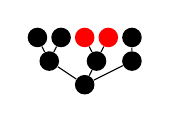
\begin{tikzpicture}[scale=.2]
      \node[circle, scale=0.75, fill] (tid0) at (3.75,0){};
      \node[circle, scale=0.75, fill] (tid1) at (1.5,1.5){};
      \node[circle, scale=0.75, fill] (tid4) at (0.75,3){};
      \node[circle, scale=0.75, fill] (tid5) at (2.25,3){};
      \draw[](tid1) -- (tid4);
      \draw[](tid1) -- (tid5);
      \node[circle, scale=0.75, fill] (tid2) at (4.5,1.5){};
      \node[circle, scale=0.75, fill, red] (tid6) at (3.75,3){};
      \node[circle, scale=0.75, fill, red] (tid7) at (5.25,3){};
      \draw[](tid2) -- (tid6);
      \draw[](tid2) -- (tid7);
      \node[circle, scale=0.75, fill] (tid3) at (6.75,1.5){};
      \node[circle, scale=0.75, fill] (tid8) at (6.75,3){};
      \draw[](tid3) -- (tid8);
      \draw[](tid0) -- (tid1);
      \draw[](tid0) -- (tid2);
      \draw[](tid0) -- (tid3);

    \end{tikzpicture}
  };
  \node[draw=black] (sn0x94ebf58W36) at (36, -30) {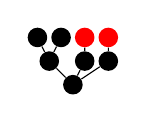
\begin{tikzpicture}[scale=.2]
      \node[circle, scale=0.75, fill] (tid0) at (3,0){};
      \node[circle, scale=0.75, fill] (tid1) at (1.5,1.5){};
      \node[circle, scale=0.75, fill] (tid4) at (0.75,3){};
      \node[circle, scale=0.75, fill] (tid5) at (2.25,3){};
      \draw[](tid1) -- (tid4);
      \draw[](tid1) -- (tid5);
      \node[circle, scale=0.75, fill] (tid2) at (3.75,1.5){};
      \node[circle, scale=0.75, fill, red] (tid6) at (3.75,3){};
      \draw[](tid2) -- (tid6);
      \node[circle, scale=0.75, fill] (tid3) at (5.25,1.5){};
      \node[circle, scale=0.75, fill, red] (tid7) at (5.25,3){};
      \draw[](tid3) -- (tid7);
      \draw[](tid0) -- (tid1);
      \draw[](tid0) -- (tid2);
      \draw[](tid0) -- (tid3);

    \end{tikzpicture}
  };
  \draw (sn0x94ebf58W36.south) -- (sn0x94ea520W36.north);
  \draw (sn0x94e4428W18.south) -- (sn0x94e66c8W9.north);
  \draw (sn0x94e4428W18.south) -- (sn0x94ebf58W36.north);
  \node[draw=black] (sn0x94e6cd8W27) at (27, -20) {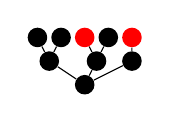
\begin{tikzpicture}[scale=.2]
      \node[circle, scale=0.75, fill] (tid0) at (3.75,0){};
      \node[circle, scale=0.75, fill] (tid1) at (1.5,1.5){};
      \node[circle, scale=0.75, fill] (tid4) at (0.75,3){};
      \node[circle, scale=0.75, fill] (tid5) at (2.25,3){};
      \draw[](tid1) -- (tid4);
      \draw[](tid1) -- (tid5);
      \node[circle, scale=0.75, fill] (tid2) at (4.5,1.5){};
      \node[circle, scale=0.75, fill, red] (tid6) at (3.75,3){};
      \node[circle, scale=0.75, fill] (tid7) at (5.25,3){};
      \draw[](tid2) -- (tid6);
      \draw[](tid2) -- (tid7);
      \node[circle, scale=0.75, fill] (tid3) at (6.75,1.5){};
      \node[circle, scale=0.75, fill, red] (tid8) at (6.75,3){};
      \draw[](tid3) -- (tid8);
      \draw[](tid0) -- (tid1);
      \draw[](tid0) -- (tid2);
      \draw[](tid0) -- (tid3);

    \end{tikzpicture}
  };
  \node[draw=black] (sn0x94ec1b0W45) at (45, -30) {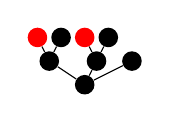
\begin{tikzpicture}[scale=.2]
      \node[circle, scale=0.75, fill] (tid0) at (3.75,0){};
      \node[circle, scale=0.75, fill] (tid1) at (1.5,1.5){};
      \node[circle, scale=0.75, fill, red] (tid4) at (0.75,3){};
      \node[circle, scale=0.75, fill] (tid5) at (2.25,3){};
      \draw[](tid1) -- (tid4);
      \draw[](tid1) -- (tid5);
      \node[circle, scale=0.75, fill] (tid2) at (4.5,1.5){};
      \node[circle, scale=0.75, fill, red] (tid6) at (3.75,3){};
      \node[circle, scale=0.75, fill] (tid7) at (5.25,3){};
      \draw[](tid2) -- (tid6);
      \draw[](tid2) -- (tid7);
      \node[circle, scale=0.75, fill] (tid3) at (6.75,1.5){};
      \draw[](tid0) -- (tid1);
      \draw[](tid0) -- (tid2);
      \draw[](tid0) -- (tid3);

    \end{tikzpicture}
  };
  \draw (sn0x94ec1b0W45.south) -- (sn0x94ea520W36.north);
  \draw (sn0x94ec1b0W45.south) -- (sn0x94ea4b8W27.north);
  \node[draw=black] (sn0x94ec4c0W54) at (54, -30) {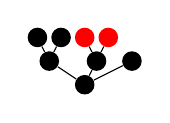
\begin{tikzpicture}[scale=.2]
      \node[circle, scale=0.75, fill] (tid0) at (3.75,0){};
      \node[circle, scale=0.75, fill] (tid1) at (1.5,1.5){};
      \node[circle, scale=0.75, fill] (tid4) at (0.75,3){};
      \node[circle, scale=0.75, fill] (tid5) at (2.25,3){};
      \draw[](tid1) -- (tid4);
      \draw[](tid1) -- (tid5);
      \node[circle, scale=0.75, fill] (tid2) at (4.5,1.5){};
      \node[circle, scale=0.75, fill, red] (tid6) at (3.75,3){};
      \node[circle, scale=0.75, fill, red] (tid7) at (5.25,3){};
      \draw[](tid2) -- (tid6);
      \draw[](tid2) -- (tid7);
      \node[circle, scale=0.75, fill] (tid3) at (6.75,1.5){};
      \draw[](tid0) -- (tid1);
      \draw[](tid0) -- (tid2);
      \draw[](tid0) -- (tid3);

    \end{tikzpicture}
  };
  \draw (sn0x94ec4c0W54.south) -- (sn0x94ea520W36.north);
  \draw (sn0x94e6cd8W27.south) -- (sn0x94e6108W27.north);
  \draw (sn0x94e6cd8W27.south) -- (sn0x94ebf58W36.north);
  \draw (sn0x94e6cd8W27.south) -- (sn0x94ec1b0W45.north);
  \draw (sn0x94e6cd8W27.south) -- (sn0x94ec4c0W54.north);
  \node[draw=black] (sn0x94e4c98W36) at (36, -20) {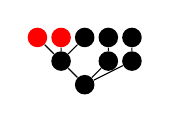
\begin{tikzpicture}[scale=.2]
      \node[circle, scale=0.75, fill] (tid0) at (3.75,0){};
      \node[circle, scale=0.75, fill] (tid1) at (2.25,1.5){};
      \node[circle, scale=0.75, fill, red] (tid4) at (0.75,3){};
      \node[circle, scale=0.75, fill, red] (tid5) at (2.25,3){};
      \node[circle, scale=0.75, fill] (tid6) at (3.75,3){};
      \draw[](tid1) -- (tid4);
      \draw[](tid1) -- (tid5);
      \draw[](tid1) -- (tid6);
      \node[circle, scale=0.75, fill] (tid2) at (5.25,1.5){};
      \node[circle, scale=0.75, fill] (tid7) at (5.25,3){};
      \draw[](tid2) -- (tid7);
      \node[circle, scale=0.75, fill] (tid3) at (6.75,1.5){};
      \node[circle, scale=0.75, fill] (tid8) at (6.75,3){};
      \draw[](tid3) -- (tid8);
      \draw[](tid0) -- (tid1);
      \draw[](tid0) -- (tid2);
      \draw[](tid0) -- (tid3);

    \end{tikzpicture}
  };
  \draw (sn0x94e4c98W36.south) -- (sn0x94e5588W18.north);
  \draw (sn0x94e4c98W36.south) -- (sn0x94e66c8W9.north);
  \draw (sn0x94e4c98W36.south) -- (sn0x94e6108W27.north);
  \node[draw=black] (sn0x94e67e0W45) at (45, -20) {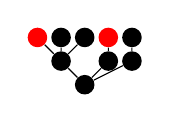
\begin{tikzpicture}[scale=.2]
      \node[circle, scale=0.75, fill] (tid0) at (3.75,0){};
      \node[circle, scale=0.75, fill] (tid1) at (2.25,1.5){};
      \node[circle, scale=0.75, fill, red] (tid4) at (0.75,3){};
      \node[circle, scale=0.75, fill] (tid5) at (2.25,3){};
      \node[circle, scale=0.75, fill] (tid6) at (3.75,3){};
      \draw[](tid1) -- (tid4);
      \draw[](tid1) -- (tid5);
      \draw[](tid1) -- (tid6);
      \node[circle, scale=0.75, fill] (tid2) at (5.25,1.5){};
      \node[circle, scale=0.75, fill, red] (tid7) at (5.25,3){};
      \draw[](tid2) -- (tid7);
      \node[circle, scale=0.75, fill] (tid3) at (6.75,1.5){};
      \node[circle, scale=0.75, fill] (tid8) at (6.75,3){};
      \draw[](tid3) -- (tid8);
      \draw[](tid0) -- (tid1);
      \draw[](tid0) -- (tid2);
      \draw[](tid0) -- (tid3);

    \end{tikzpicture}
  };
  \node[draw=black] (sn0x94ec8b0W63) at (63, -30) {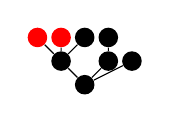
\begin{tikzpicture}[scale=.2]
      \node[circle, scale=0.75, fill] (tid0) at (3.75,0){};
      \node[circle, scale=0.75, fill] (tid1) at (2.25,1.5){};
      \node[circle, scale=0.75, fill, red] (tid4) at (0.75,3){};
      \node[circle, scale=0.75, fill, red] (tid5) at (2.25,3){};
      \node[circle, scale=0.75, fill] (tid6) at (3.75,3){};
      \draw[](tid1) -- (tid4);
      \draw[](tid1) -- (tid5);
      \draw[](tid1) -- (tid6);
      \node[circle, scale=0.75, fill] (tid2) at (5.25,1.5){};
      \node[circle, scale=0.75, fill] (tid7) at (5.25,3){};
      \draw[](tid2) -- (tid7);
      \node[circle, scale=0.75, fill] (tid3) at (6.75,1.5){};
      \draw[](tid0) -- (tid1);
      \draw[](tid0) -- (tid2);
      \draw[](tid0) -- (tid3);

    \end{tikzpicture}
  };
  \draw (sn0x94ec8b0W63.south) -- (sn0x94ea4b8W27.north);
  \draw (sn0x94ec8b0W63.south) -- (sn0x94ea520W36.north);
  \node[draw=black] (sn0x94ecc50W72) at (72, -30) {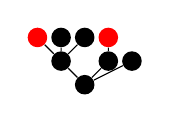
\begin{tikzpicture}[scale=.2]
      \node[circle, scale=0.75, fill] (tid0) at (3.75,0){};
      \node[circle, scale=0.75, fill] (tid1) at (2.25,1.5){};
      \node[circle, scale=0.75, fill, red] (tid4) at (0.75,3){};
      \node[circle, scale=0.75, fill] (tid5) at (2.25,3){};
      \node[circle, scale=0.75, fill] (tid6) at (3.75,3){};
      \draw[](tid1) -- (tid4);
      \draw[](tid1) -- (tid5);
      \draw[](tid1) -- (tid6);
      \node[circle, scale=0.75, fill] (tid2) at (5.25,1.5){};
      \node[circle, scale=0.75, fill, red] (tid7) at (5.25,3){};
      \draw[](tid2) -- (tid7);
      \node[circle, scale=0.75, fill] (tid3) at (6.75,1.5){};
      \draw[](tid0) -- (tid1);
      \draw[](tid0) -- (tid2);
      \draw[](tid0) -- (tid3);

    \end{tikzpicture}
  };
  \node[draw=black] (sn0x94ece48W54) at (54, -40) {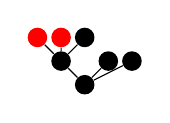
\begin{tikzpicture}[scale=.2]
      \node[circle, scale=0.75, fill] (tid0) at (3.75,0){};
      \node[circle, scale=0.75, fill] (tid1) at (2.25,1.5){};
      \node[circle, scale=0.75, fill, red] (tid4) at (0.75,3){};
      \node[circle, scale=0.75, fill, red] (tid5) at (2.25,3){};
      \node[circle, scale=0.75, fill] (tid6) at (3.75,3){};
      \draw[](tid1) -- (tid4);
      \draw[](tid1) -- (tid5);
      \draw[](tid1) -- (tid6);
      \node[circle, scale=0.75, fill] (tid2) at (5.25,1.5){};
      \node[circle, scale=0.75, fill] (tid3) at (6.75,1.5){};
      \draw[](tid0) -- (tid1);
      \draw[](tid0) -- (tid2);
      \draw[](tid0) -- (tid3);

    \end{tikzpicture}
  };
  \draw (sn0x94ece48W54.south) -- (sn0x94eb378W18.north);
  \draw (sn0x94ecc50W72.south) -- (sn0x94ea520W36.north);
  \draw (sn0x94ecc50W72.south) -- (sn0x94ece48W54.north);
  \draw (sn0x94e67e0W45.south) -- (sn0x94e66c8W9.north);
  \draw (sn0x94e67e0W45.south) -- (sn0x94ebf58W36.north);
  \draw (sn0x94e67e0W45.south) -- (sn0x94ec8b0W63.north);
  \draw (sn0x94e67e0W45.south) -- (sn0x94ecc50W72.north);
  \node[draw=black] (sn0x94e6aa8W54) at (54, -20) {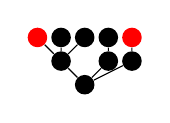
\begin{tikzpicture}[scale=.2]
      \node[circle, scale=0.75, fill] (tid0) at (3.75,0){};
      \node[circle, scale=0.75, fill] (tid1) at (2.25,1.5){};
      \node[circle, scale=0.75, fill, red] (tid4) at (0.75,3){};
      \node[circle, scale=0.75, fill] (tid5) at (2.25,3){};
      \node[circle, scale=0.75, fill] (tid6) at (3.75,3){};
      \draw[](tid1) -- (tid4);
      \draw[](tid1) -- (tid5);
      \draw[](tid1) -- (tid6);
      \node[circle, scale=0.75, fill] (tid2) at (5.25,1.5){};
      \node[circle, scale=0.75, fill] (tid7) at (5.25,3){};
      \draw[](tid2) -- (tid7);
      \node[circle, scale=0.75, fill] (tid3) at (6.75,1.5){};
      \node[circle, scale=0.75, fill, red] (tid8) at (6.75,3){};
      \draw[](tid3) -- (tid8);
      \draw[](tid0) -- (tid1);
      \draw[](tid0) -- (tid2);
      \draw[](tid0) -- (tid3);

    \end{tikzpicture}
  };
  \draw (sn0x94e6aa8W54.south) -- (sn0x94e6108W27.north);
  \draw (sn0x94e6aa8W54.south) -- (sn0x94ebf58W36.north);
  \draw (sn0x94e6aa8W54.south) -- (sn0x94ec8b0W63.north);
  \draw (sn0x94e6aa8W54.south) -- (sn0x94ecc50W72.north);
  \draw (sn0x94e5990W9.south) -- (sn0x94e5730W9.north);
  \draw (sn0x94e5990W9.south) -- (sn0x94e4428W18.north);
  \draw (sn0x94e5990W9.south) -- (sn0x94e6cd8W27.north);
  \draw (sn0x94e5990W9.south) -- (sn0x94e4c98W36.north);
  \draw (sn0x94e5990W9.south) -- (sn0x94e67e0W45.north);
  \draw (sn0x94e5990W9.south) -- (sn0x94e6aa8W54.north);
\end{tikzpicture}

%%% Local Variables:
%%% TeX-master: "thesis/thesis.tex"
%%% End: 

\begin{tikzpicture}[scale=.2, anchor=base]
\node[draw=black] (sn0x94e59f0W9) at (9, -10) {\begin{tikzpicture}[scale=.2]
\node[circle, scale=0.75, fill] (tid0) at (4.5,0){};
\node[circle, scale=0.75, fill] (tid1) at (2.25,1.5){};
\node[circle, scale=0.75, fill, red] (tid4) at (0.75,3){};
\node[circle, scale=0.75, fill, red] (tid5) at (2.25,3){};
\node[circle, scale=0.75, fill] (tid6) at (3.75,3){};
\draw[](tid1) -- (tid4);
\draw[](tid1) -- (tid5);
\draw[](tid1) -- (tid6);
\node[circle, scale=0.75, fill] (tid2) at (6,1.5){};
\node[circle, scale=0.75, fill] (tid7) at (5.25,3){};
\node[circle, scale=0.75, fill] (tid8) at (6.75,3){};
\draw[](tid2) -- (tid7);
\draw[](tid2) -- (tid8);
\node[circle, scale=0.75, fill] (tid3) at (8.25,1.5){};
\node[circle, scale=0.75, fill] (tid9) at (8.25,3){};
\draw[](tid3) -- (tid9);
\draw[](tid0) -- (tid1);
\draw[](tid0) -- (tid2);
\draw[](tid0) -- (tid3);

\end{tikzpicture}
};
\node[draw=black] (sn0x94ed650W9) at (9, -20) {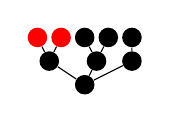
\begin{tikzpicture}[scale=.2]
\node[circle, scale=0.75, fill] (tid0) at (3.75,0){};
\node[circle, scale=0.75, fill] (tid1) at (1.5,1.5){};
\node[circle, scale=0.75, fill, red] (tid4) at (0.75,3){};
\node[circle, scale=0.75, fill, red] (tid5) at (2.25,3){};
\draw[](tid1) -- (tid4);
\draw[](tid1) -- (tid5);
\node[circle, scale=0.75, fill] (tid2) at (4.5,1.5){};
\node[circle, scale=0.75, fill] (tid6) at (3.75,3){};
\node[circle, scale=0.75, fill] (tid7) at (5.25,3){};
\draw[](tid2) -- (tid6);
\draw[](tid2) -- (tid7);
\node[circle, scale=0.75, fill] (tid3) at (6.75,1.5){};
\node[circle, scale=0.75, fill] (tid8) at (6.75,3){};
\draw[](tid3) -- (tid8);
\draw[](tid0) -- (tid1);
\draw[](tid0) -- (tid2);
\draw[](tid0) -- (tid3);

\end{tikzpicture}
};
\node[draw=black] (sn0x94e66c8W9) at (9, -30) {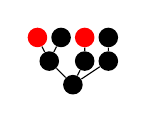
\begin{tikzpicture}[scale=.2]
\node[circle, scale=0.75, fill] (tid0) at (3,0){};
\node[circle, scale=0.75, fill] (tid1) at (1.5,1.5){};
\node[circle, scale=0.75, fill, red] (tid4) at (0.75,3){};
\node[circle, scale=0.75, fill] (tid5) at (2.25,3){};
\draw[](tid1) -- (tid4);
\draw[](tid1) -- (tid5);
\node[circle, scale=0.75, fill] (tid2) at (3.75,1.5){};
\node[circle, scale=0.75, fill, red] (tid6) at (3.75,3){};
\draw[](tid2) -- (tid6);
\node[circle, scale=0.75, fill] (tid3) at (5.25,1.5){};
\node[circle, scale=0.75, fill] (tid7) at (5.25,3){};
\draw[](tid3) -- (tid7);
\draw[](tid0) -- (tid1);
\draw[](tid0) -- (tid2);
\draw[](tid0) -- (tid3);

\end{tikzpicture}
};
\node[draw=black] (sn0x94e9fd8W9) at (9, -40) {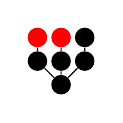
\begin{tikzpicture}[scale=.2]
\node[circle, scale=0.75, fill] (tid0) at (2.25,0){};
\node[circle, scale=0.75, fill] (tid1) at (0.75,1.5){};
\node[circle, scale=0.75, fill, red] (tid4) at (0.75,3){};
\draw[](tid1) -- (tid4);
\node[circle, scale=0.75, fill] (tid2) at (2.25,1.5){};
\node[circle, scale=0.75, fill, red] (tid5) at (2.25,3){};
\draw[](tid2) -- (tid5);
\node[circle, scale=0.75, fill] (tid3) at (3.75,1.5){};
\node[circle, scale=0.75, fill] (tid6) at (3.75,3){};
\draw[](tid3) -- (tid6);
\draw[](tid0) -- (tid1);
\draw[](tid0) -- (tid2);
\draw[](tid0) -- (tid3);

\end{tikzpicture}
};
\node[draw=black] (sn0x94ea750W9) at (9, -50) {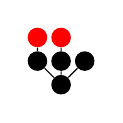
\begin{tikzpicture}[scale=.2]
\node[circle, scale=0.75, fill] (tid0) at (2.25,0){};
\node[circle, scale=0.75, fill] (tid1) at (0.75,1.5){};
\node[circle, scale=0.75, fill, red] (tid4) at (0.75,3){};
\draw[](tid1) -- (tid4);
\node[circle, scale=0.75, fill] (tid2) at (2.25,1.5){};
\node[circle, scale=0.75, fill, red] (tid5) at (2.25,3){};
\draw[](tid2) -- (tid5);
\node[circle, scale=0.75, fill] (tid3) at (3.75,1.5){};
\draw[](tid0) -- (tid1);
\draw[](tid0) -- (tid2);
\draw[](tid0) -- (tid3);

\end{tikzpicture}
};
\node[draw=black] (sn0x94eaa10W9) at (9, -60) {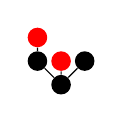
\begin{tikzpicture}[scale=.2]
\node[circle, scale=0.75, fill] (tid0) at (2.25,0){};
\node[circle, scale=0.75, fill] (tid1) at (0.75,1.5){};
\node[circle, scale=0.75, fill, red] (tid4) at (0.75,3){};
\draw[](tid1) -- (tid4);
\node[circle, scale=0.75, fill, red] (tid2) at (2.25,1.5){};
\node[circle, scale=0.75, fill] (tid3) at (3.75,1.5){};
\draw[](tid0) -- (tid1);
\draw[](tid0) -- (tid2);
\draw[](tid0) -- (tid3);

\end{tikzpicture}
};
\node[draw=black] (sn0x94ea990W9) at (9, -70) {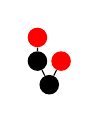
\begin{tikzpicture}[scale=.2]
\node[circle, scale=0.75, fill] (tid0) at (1.5,0){};
\node[circle, scale=0.75, fill] (tid1) at (0.75,1.5){};
\node[circle, scale=0.75, fill, red] (tid3) at (0.75,3){};
\draw[](tid1) -- (tid3);
\node[circle, scale=0.75, fill, red] (tid2) at (2.25,1.5){};
\draw[](tid0) -- (tid1);
\draw[](tid0) -- (tid2);

\end{tikzpicture}
};
\node[draw=black] (sn0x94ead40W9) at (9, -80) {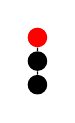
\begin{tikzpicture}[scale=.2]
\node[circle, scale=0.75, fill] (tid0) at (0.75,0){};
\node[circle, scale=0.75, fill] (tid1) at (0.75,1.5){};
\node[circle, scale=0.75, fill, red] (tid2) at (0.75,3){};
\draw[](tid1) -- (tid2);
\draw[](tid0) -- (tid1);

\end{tikzpicture}
};
\node[draw=black] (sn0x94eb148W9) at (9, -90) {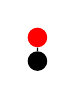
\begin{tikzpicture}[scale=.2]
\node[circle, scale=0.75, fill] (tid0) at (0.75,0){};
\node[circle, scale=0.75, fill, red] (tid1) at (0.75,1.5){};
\draw[](tid0) -- (tid1);

\end{tikzpicture}
};
\node[draw=black] (sn0x94eb1b0W9) at (9, -100) {
\begin{tikzpicture}[scale=.2]
\node[circle, scale=0.75, fill, red] (tid0) at (0.75,0){};

\end{tikzpicture}
};
\draw (sn0x94eb148W9.south) -- (sn0x94eb1b0W9.north);
\draw (sn0x94ead40W9.south) -- (sn0x94eb148W9.north);
\node[draw=black] (sn0x94eaff8W18) at (18, -80) {
\begin{tikzpicture}[scale=.2]
\node[circle, scale=0.75, fill] (tid0) at (1.5,0){};
\node[circle, scale=0.75, fill, red] (tid1) at (0.75,1.5){};
\node[circle, scale=0.75, fill, red] (tid2) at (2.25,1.5){};
\draw[](tid0) -- (tid1);
\draw[](tid0) -- (tid2);

\end{tikzpicture}
};
\draw (sn0x94eaff8W18.south) -- (sn0x94eb148W9.north);
\draw (sn0x94ea990W9.south) -- (sn0x94ead40W9.north);
\draw (sn0x94ea990W9.south) -- (sn0x94eaff8W18.north);
\node[draw=black] (sn0x94eacd8W18) at (18, -70) {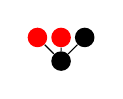
\begin{tikzpicture}[scale=.2]
\node[circle, scale=0.75, fill] (tid0) at (2.25,0){};
\node[circle, scale=0.75, fill, red] (tid1) at (0.75,1.5){};
\node[circle, scale=0.75, fill, red] (tid2) at (2.25,1.5){};
\node[circle, scale=0.75, fill] (tid3) at (3.75,1.5){};
\draw[](tid0) -- (tid1);
\draw[](tid0) -- (tid2);
\draw[](tid0) -- (tid3);

\end{tikzpicture}
};
\draw (sn0x94eacd8W18.south) -- (sn0x94eaff8W18.north);
\draw (sn0x94eaa10W9.south) -- (sn0x94ea990W9.north);
\draw (sn0x94eaa10W9.south) -- (sn0x94eacd8W18.north);
\draw (sn0x94ea750W9.south) -- (sn0x94eaa10W9.north);
\draw (sn0x94e9fd8W9.south) -- (sn0x94ea750W9.north);
\node[draw=black] (sn0x94ea1a0W18) at (18, -40) {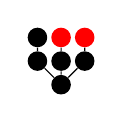
\begin{tikzpicture}[scale=.2]
\node[circle, scale=0.75, fill] (tid0) at (2.25,0){};
\node[circle, scale=0.75, fill] (tid1) at (0.75,1.5){};
\node[circle, scale=0.75, fill] (tid4) at (0.75,3){};
\draw[](tid1) -- (tid4);
\node[circle, scale=0.75, fill] (tid2) at (2.25,1.5){};
\node[circle, scale=0.75, fill, red] (tid5) at (2.25,3){};
\draw[](tid2) -- (tid5);
\node[circle, scale=0.75, fill] (tid3) at (3.75,1.5){};
\node[circle, scale=0.75, fill, red] (tid6) at (3.75,3){};
\draw[](tid3) -- (tid6);
\draw[](tid0) -- (tid1);
\draw[](tid0) -- (tid2);
\draw[](tid0) -- (tid3);

\end{tikzpicture}
};
\draw (sn0x94ea1a0W18.south) -- (sn0x94ea750W9.north);
\node[draw=black] (sn0x94ea4b8W27) at (27, -40) {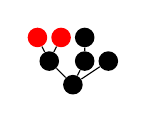
\begin{tikzpicture}[scale=.2]
\node[circle, scale=0.75, fill] (tid0) at (3,0){};
\node[circle, scale=0.75, fill] (tid1) at (1.5,1.5){};
\node[circle, scale=0.75, fill, red] (tid4) at (0.75,3){};
\node[circle, scale=0.75, fill, red] (tid5) at (2.25,3){};
\draw[](tid1) -- (tid4);
\draw[](tid1) -- (tid5);
\node[circle, scale=0.75, fill] (tid2) at (3.75,1.5){};
\node[circle, scale=0.75, fill] (tid6) at (3.75,3){};
\draw[](tid2) -- (tid6);
\node[circle, scale=0.75, fill] (tid3) at (5.25,1.5){};
\draw[](tid0) -- (tid1);
\draw[](tid0) -- (tid2);
\draw[](tid0) -- (tid3);

\end{tikzpicture}
};
\draw (sn0x94ea4b8W27.south) -- (sn0x94ea750W9.north);
\node[draw=black] (sn0x94ea520W36) at (36, -40) {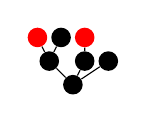
\begin{tikzpicture}[scale=.2]
\node[circle, scale=0.75, fill] (tid0) at (3,0){};
\node[circle, scale=0.75, fill] (tid1) at (1.5,1.5){};
\node[circle, scale=0.75, fill, red] (tid4) at (0.75,3){};
\node[circle, scale=0.75, fill] (tid5) at (2.25,3){};
\draw[](tid1) -- (tid4);
\draw[](tid1) -- (tid5);
\node[circle, scale=0.75, fill] (tid2) at (3.75,1.5){};
\node[circle, scale=0.75, fill, red] (tid6) at (3.75,3){};
\draw[](tid2) -- (tid6);
\node[circle, scale=0.75, fill] (tid3) at (5.25,1.5){};
\draw[](tid0) -- (tid1);
\draw[](tid0) -- (tid2);
\draw[](tid0) -- (tid3);

\end{tikzpicture}
};
\node[draw=black] (sn0x94eb378W18) at (18, -50) {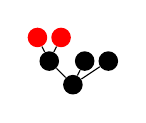
\begin{tikzpicture}[scale=.2]
\node[circle, scale=0.75, fill] (tid0) at (3,0){};
\node[circle, scale=0.75, fill] (tid1) at (1.5,1.5){};
\node[circle, scale=0.75, fill, red] (tid4) at (0.75,3){};
\node[circle, scale=0.75, fill, red] (tid5) at (2.25,3){};
\draw[](tid1) -- (tid4);
\draw[](tid1) -- (tid5);
\node[circle, scale=0.75, fill] (tid2) at (3.75,1.5){};
\node[circle, scale=0.75, fill] (tid3) at (5.25,1.5){};
\draw[](tid0) -- (tid1);
\draw[](tid0) -- (tid2);
\draw[](tid0) -- (tid3);

\end{tikzpicture}
};
\draw (sn0x94eb378W18.south) -- (sn0x94eaa10W9.north);
\draw (sn0x94ea520W36.south) -- (sn0x94ea750W9.north);
\draw (sn0x94ea520W36.south) -- (sn0x94eb378W18.north);
\draw (sn0x94e66c8W9.south) -- (sn0x94e9fd8W9.north);
\draw (sn0x94e66c8W9.south) -- (sn0x94ea1a0W18.north);
\draw (sn0x94e66c8W9.south) -- (sn0x94ea4b8W27.north);
\draw (sn0x94e66c8W9.south) -- (sn0x94ea520W36.north);
\node[draw=black] (sn0x94ebf58W18) at (18, -30) {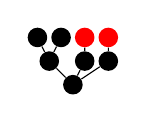
\begin{tikzpicture}[scale=.2]
\node[circle, scale=0.75, fill] (tid0) at (3,0){};
\node[circle, scale=0.75, fill] (tid1) at (1.5,1.5){};
\node[circle, scale=0.75, fill] (tid4) at (0.75,3){};
\node[circle, scale=0.75, fill] (tid5) at (2.25,3){};
\draw[](tid1) -- (tid4);
\draw[](tid1) -- (tid5);
\node[circle, scale=0.75, fill] (tid2) at (3.75,1.5){};
\node[circle, scale=0.75, fill, red] (tid6) at (3.75,3){};
\draw[](tid2) -- (tid6);
\node[circle, scale=0.75, fill] (tid3) at (5.25,1.5){};
\node[circle, scale=0.75, fill, red] (tid7) at (5.25,3){};
\draw[](tid3) -- (tid7);
\draw[](tid0) -- (tid1);
\draw[](tid0) -- (tid2);
\draw[](tid0) -- (tid3);

\end{tikzpicture}
};
\draw (sn0x94ebf58W18.south) -- (sn0x94ea520W36.north);
\draw (sn0x94ed650W9.south) -- (sn0x94e66c8W9.north);
\draw (sn0x94ed650W9.south) -- (sn0x94ebf58W18.north);
\node[draw=black] (sn0x94e5730W18) at (18, -20) {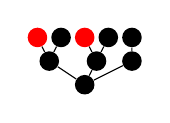
\begin{tikzpicture}[scale=.2]
\node[circle, scale=0.75, fill] (tid0) at (3.75,0){};
\node[circle, scale=0.75, fill] (tid1) at (1.5,1.5){};
\node[circle, scale=0.75, fill, red] (tid4) at (0.75,3){};
\node[circle, scale=0.75, fill] (tid5) at (2.25,3){};
\draw[](tid1) -- (tid4);
\draw[](tid1) -- (tid5);
\node[circle, scale=0.75, fill] (tid2) at (4.5,1.5){};
\node[circle, scale=0.75, fill, red] (tid6) at (3.75,3){};
\node[circle, scale=0.75, fill] (tid7) at (5.25,3){};
\draw[](tid2) -- (tid6);
\draw[](tid2) -- (tid7);
\node[circle, scale=0.75, fill] (tid3) at (6.75,1.5){};
\node[circle, scale=0.75, fill] (tid8) at (6.75,3){};
\draw[](tid3) -- (tid8);
\draw[](tid0) -- (tid1);
\draw[](tid0) -- (tid2);
\draw[](tid0) -- (tid3);

\end{tikzpicture}
};
\node[draw=black] (sn0x94e5588W27) at (27, -30) {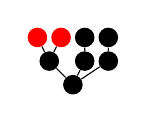
\begin{tikzpicture}[scale=.2]
\node[circle, scale=0.75, fill] (tid0) at (3,0){};
\node[circle, scale=0.75, fill] (tid1) at (1.5,1.5){};
\node[circle, scale=0.75, fill, red] (tid4) at (0.75,3){};
\node[circle, scale=0.75, fill, red] (tid5) at (2.25,3){};
\draw[](tid1) -- (tid4);
\draw[](tid1) -- (tid5);
\node[circle, scale=0.75, fill] (tid2) at (3.75,1.5){};
\node[circle, scale=0.75, fill] (tid6) at (3.75,3){};
\draw[](tid2) -- (tid6);
\node[circle, scale=0.75, fill] (tid3) at (5.25,1.5){};
\node[circle, scale=0.75, fill] (tid7) at (5.25,3){};
\draw[](tid3) -- (tid7);
\draw[](tid0) -- (tid1);
\draw[](tid0) -- (tid2);
\draw[](tid0) -- (tid3);

\end{tikzpicture}
};
\node[draw=black] (sn0x94ebd08W45) at (45, -40) {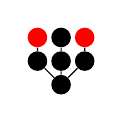
\begin{tikzpicture}[scale=.2]
\node[circle, scale=0.75, fill] (tid0) at (2.25,0){};
\node[circle, scale=0.75, fill] (tid1) at (0.75,1.5){};
\node[circle, scale=0.75, fill, red] (tid4) at (0.75,3){};
\draw[](tid1) -- (tid4);
\node[circle, scale=0.75, fill] (tid2) at (2.25,1.5){};
\node[circle, scale=0.75, fill] (tid5) at (2.25,3){};
\draw[](tid2) -- (tid5);
\node[circle, scale=0.75, fill] (tid3) at (3.75,1.5){};
\node[circle, scale=0.75, fill, red] (tid6) at (3.75,3){};
\draw[](tid3) -- (tid6);
\draw[](tid0) -- (tid1);
\draw[](tid0) -- (tid2);
\draw[](tid0) -- (tid3);

\end{tikzpicture}
};
\draw (sn0x94ebd08W45.south) -- (sn0x94ea750W9.north);
\draw (sn0x94e5588W27.south) -- (sn0x94e9fd8W9.north);
\draw (sn0x94e5588W27.south) -- (sn0x94ebd08W45.north);
\node[draw=black] (sn0x94e6108W36) at (36, -30) {\begin{tikzpicture}[scale=.2]
\node[circle, scale=0.75, fill] (tid0) at (3,0){};
\node[circle, scale=0.75, fill] (tid1) at (1.5,1.5){};
\node[circle, scale=0.75, fill, red] (tid4) at (0.75,3){};
\node[circle, scale=0.75, fill] (tid5) at (2.25,3){};
\draw[](tid1) -- (tid4);
\draw[](tid1) -- (tid5);
\node[circle, scale=0.75, fill] (tid2) at (3.75,1.5){};
\node[circle, scale=0.75, fill] (tid6) at (3.75,3){};
\draw[](tid2) -- (tid6);
\node[circle, scale=0.75, fill] (tid3) at (5.25,1.5){};
\node[circle, scale=0.75, fill, red] (tid7) at (5.25,3){};
\draw[](tid3) -- (tid7);
\draw[](tid0) -- (tid1);
\draw[](tid0) -- (tid2);
\draw[](tid0) -- (tid3);

\end{tikzpicture}
};
\draw (sn0x94e6108W36.south) -- (sn0x94ebd08W45.north);
\draw (sn0x94e6108W36.south) -- (sn0x94ea1a0W18.north);
\draw (sn0x94e6108W36.south) -- (sn0x94ea4b8W27.north);
\draw (sn0x94e6108W36.south) -- (sn0x94ea520W36.north);
\draw (sn0x94e5730W18.south) -- (sn0x94e66c8W9.north);
\draw (sn0x94e5730W18.south) -- (sn0x94e5588W27.north);
\draw (sn0x94e5730W18.south) -- (sn0x94e6108W36.north);
\node[draw=black] (sn0x94ed7b0W27) at (27, -20) {\begin{tikzpicture}[scale=.2]
\node[circle, scale=0.75, fill] (tid0) at (3.75,0){};
\node[circle, scale=0.75, fill] (tid1) at (1.5,1.5){};
\node[circle, scale=0.75, fill, red] (tid4) at (0.75,3){};
\node[circle, scale=0.75, fill] (tid5) at (2.25,3){};
\draw[](tid1) -- (tid4);
\draw[](tid1) -- (tid5);
\node[circle, scale=0.75, fill] (tid2) at (4.5,1.5){};
\node[circle, scale=0.75, fill] (tid6) at (3.75,3){};
\node[circle, scale=0.75, fill] (tid7) at (5.25,3){};
\draw[](tid2) -- (tid6);
\draw[](tid2) -- (tid7);
\node[circle, scale=0.75, fill] (tid3) at (6.75,1.5){};
\node[circle, scale=0.75, fill, red] (tid8) at (6.75,3){};
\draw[](tid3) -- (tid8);
\draw[](tid0) -- (tid1);
\draw[](tid0) -- (tid2);
\draw[](tid0) -- (tid3);

\end{tikzpicture}
};
\node[draw=black] (sn0x94edb78W45) at (45, -30) {\begin{tikzpicture}[scale=.2]
\node[circle, scale=0.75, fill] (tid0) at (3.75,0){};
\node[circle, scale=0.75, fill] (tid1) at (1.5,1.5){};
\node[circle, scale=0.75, fill, red] (tid4) at (0.75,3){};
\node[circle, scale=0.75, fill, red] (tid5) at (2.25,3){};
\draw[](tid1) -- (tid4);
\draw[](tid1) -- (tid5);
\node[circle, scale=0.75, fill] (tid2) at (4.5,1.5){};
\node[circle, scale=0.75, fill] (tid6) at (3.75,3){};
\node[circle, scale=0.75, fill] (tid7) at (5.25,3){};
\draw[](tid2) -- (tid6);
\draw[](tid2) -- (tid7);
\node[circle, scale=0.75, fill] (tid3) at (6.75,1.5){};
\draw[](tid0) -- (tid1);
\draw[](tid0) -- (tid2);
\draw[](tid0) -- (tid3);

\end{tikzpicture}
};
\draw (sn0x94edb78W45.south) -- (sn0x94ea520W36.north);
\node[draw=black] (sn0x94ec1b0W54) at (54, -30) {\begin{tikzpicture}[scale=.2]
\node[circle, scale=0.75, fill] (tid0) at (3.75,0){};
\node[circle, scale=0.75, fill] (tid1) at (1.5,1.5){};
\node[circle, scale=0.75, fill, red] (tid4) at (0.75,3){};
\node[circle, scale=0.75, fill] (tid5) at (2.25,3){};
\draw[](tid1) -- (tid4);
\draw[](tid1) -- (tid5);
\node[circle, scale=0.75, fill] (tid2) at (4.5,1.5){};
\node[circle, scale=0.75, fill, red] (tid6) at (3.75,3){};
\node[circle, scale=0.75, fill] (tid7) at (5.25,3){};
\draw[](tid2) -- (tid6);
\draw[](tid2) -- (tid7);
\node[circle, scale=0.75, fill] (tid3) at (6.75,1.5){};
\draw[](tid0) -- (tid1);
\draw[](tid0) -- (tid2);
\draw[](tid0) -- (tid3);

\end{tikzpicture}
};
\draw (sn0x94ec1b0W54.south) -- (sn0x94ea520W36.north);
\draw (sn0x94ec1b0W54.south) -- (sn0x94ea4b8W27.north);
\draw (sn0x94ed7b0W27.south) -- (sn0x94ebf58W18.north);
\draw (sn0x94ed7b0W27.south) -- (sn0x94e6108W36.north);
\draw (sn0x94ed7b0W27.south) -- (sn0x94edb78W45.north);
\draw (sn0x94ed7b0W27.south) -- (sn0x94ec1b0W54.north);
\draw (sn0x94e59f0W9.south) -- (sn0x94ed650W9.north);
\draw (sn0x94e59f0W9.south) -- (sn0x94e5730W18.north);
\draw (sn0x94e59f0W9.south) -- (sn0x94ed7b0W27.north);
\end{tikzpicture}

%%% Local Variables:
%%% TeX-master: "thesis/thesis.tex"
%%% End: 

\begin{tikzpicture}[scale=.2, anchor=base]
\node[draw=black] (sn0x94e5a50W9) at (9, -10) {\begin{tikzpicture}[scale=.2]
\node[circle, scale=0.75, fill] (tid0) at (4.5,0){};
\node[circle, scale=0.75, fill] (tid1) at (2.25,1.5){};
\node[circle, scale=0.75, fill, red] (tid4) at (0.75,3){};
\node[circle, scale=0.75, fill] (tid5) at (2.25,3){};
\node[circle, scale=0.75, fill] (tid6) at (3.75,3){};
\draw[](tid1) -- (tid4);
\draw[](tid1) -- (tid5);
\draw[](tid1) -- (tid6);
\node[circle, scale=0.75, fill] (tid2) at (6,1.5){};
\node[circle, scale=0.75, fill] (tid7) at (5.25,3){};
\node[circle, scale=0.75, fill] (tid8) at (6.75,3){};
\draw[](tid2) -- (tid7);
\draw[](tid2) -- (tid8);
\node[circle, scale=0.75, fill] (tid3) at (8.25,1.5){};
\node[circle, scale=0.75, fill, red] (tid9) at (8.25,3){};
\draw[](tid3) -- (tid9);
\draw[](tid0) -- (tid1);
\draw[](tid0) -- (tid2);
\draw[](tid0) -- (tid3);

\end{tikzpicture}
};
\node[draw=black] (sn0x94ed7b0W9) at (9, -20) {\begin{tikzpicture}[scale=.2]
\node[circle, scale=0.75, fill] (tid0) at (3.75,0){};
\node[circle, scale=0.75, fill] (tid1) at (1.5,1.5){};
\node[circle, scale=0.75, fill, red] (tid4) at (0.75,3){};
\node[circle, scale=0.75, fill] (tid5) at (2.25,3){};
\draw[](tid1) -- (tid4);
\draw[](tid1) -- (tid5);
\node[circle, scale=0.75, fill] (tid2) at (4.5,1.5){};
\node[circle, scale=0.75, fill] (tid6) at (3.75,3){};
\node[circle, scale=0.75, fill] (tid7) at (5.25,3){};
\draw[](tid2) -- (tid6);
\draw[](tid2) -- (tid7);
\node[circle, scale=0.75, fill] (tid3) at (6.75,1.5){};
\node[circle, scale=0.75, fill, red] (tid8) at (6.75,3){};
\draw[](tid3) -- (tid8);
\draw[](tid0) -- (tid1);
\draw[](tid0) -- (tid2);
\draw[](tid0) -- (tid3);

\end{tikzpicture}
};
\node[draw=black] (sn0x94ebf58W9) at (9, -30) {\begin{tikzpicture}[scale=.2]
\node[circle, scale=0.75, fill] (tid0) at (3,0){};
\node[circle, scale=0.75, fill] (tid1) at (1.5,1.5){};
\node[circle, scale=0.75, fill] (tid4) at (0.75,3){};
\node[circle, scale=0.75, fill] (tid5) at (2.25,3){};
\draw[](tid1) -- (tid4);
\draw[](tid1) -- (tid5);
\node[circle, scale=0.75, fill] (tid2) at (3.75,1.5){};
\node[circle, scale=0.75, fill, red] (tid6) at (3.75,3){};
\draw[](tid2) -- (tid6);
\node[circle, scale=0.75, fill] (tid3) at (5.25,1.5){};
\node[circle, scale=0.75, fill, red] (tid7) at (5.25,3){};
\draw[](tid3) -- (tid7);
\draw[](tid0) -- (tid1);
\draw[](tid0) -- (tid2);
\draw[](tid0) -- (tid3);

\end{tikzpicture}
};
\node[draw=black] (sn0x94ea520W9) at (9, -40) {\begin{tikzpicture}[scale=.2]
\node[circle, scale=0.75, fill] (tid0) at (3,0){};
\node[circle, scale=0.75, fill] (tid1) at (1.5,1.5){};
\node[circle, scale=0.75, fill, red] (tid4) at (0.75,3){};
\node[circle, scale=0.75, fill] (tid5) at (2.25,3){};
\draw[](tid1) -- (tid4);
\draw[](tid1) -- (tid5);
\node[circle, scale=0.75, fill] (tid2) at (3.75,1.5){};
\node[circle, scale=0.75, fill, red] (tid6) at (3.75,3){};
\draw[](tid2) -- (tid6);
\node[circle, scale=0.75, fill] (tid3) at (5.25,1.5){};
\draw[](tid0) -- (tid1);
\draw[](tid0) -- (tid2);
\draw[](tid0) -- (tid3);

\end{tikzpicture}
};
\node[draw=black] (sn0x94ea750W9) at (9, -50) {\begin{tikzpicture}[scale=.2]
\node[circle, scale=0.75, fill] (tid0) at (2.25,0){};
\node[circle, scale=0.75, fill] (tid1) at (0.75,1.5){};
\node[circle, scale=0.75, fill, red] (tid4) at (0.75,3){};
\draw[](tid1) -- (tid4);
\node[circle, scale=0.75, fill] (tid2) at (2.25,1.5){};
\node[circle, scale=0.75, fill, red] (tid5) at (2.25,3){};
\draw[](tid2) -- (tid5);
\node[circle, scale=0.75, fill] (tid3) at (3.75,1.5){};
\draw[](tid0) -- (tid1);
\draw[](tid0) -- (tid2);
\draw[](tid0) -- (tid3);

\end{tikzpicture}
};
\node[draw=black] (sn0x94eaa10W9) at (9, -60) {\begin{tikzpicture}[scale=.2]
\node[circle, scale=0.75, fill] (tid0) at (2.25,0){};
\node[circle, scale=0.75, fill] (tid1) at (0.75,1.5){};
\node[circle, scale=0.75, fill, red] (tid4) at (0.75,3){};
\draw[](tid1) -- (tid4);
\node[circle, scale=0.75, fill, red] (tid2) at (2.25,1.5){};
\node[circle, scale=0.75, fill] (tid3) at (3.75,1.5){};
\draw[](tid0) -- (tid1);
\draw[](tid0) -- (tid2);
\draw[](tid0) -- (tid3);

\end{tikzpicture}
};
\node[draw=black] (sn0x94ea990W9) at (9, -70) {\begin{tikzpicture}[scale=.2]
\node[circle, scale=0.75, fill] (tid0) at (1.5,0){};
\node[circle, scale=0.75, fill] (tid1) at (0.75,1.5){};
\node[circle, scale=0.75, fill, red] (tid3) at (0.75,3){};
\draw[](tid1) -- (tid3);
\node[circle, scale=0.75, fill, red] (tid2) at (2.25,1.5){};
\draw[](tid0) -- (tid1);
\draw[](tid0) -- (tid2);

\end{tikzpicture}
};
\node[draw=black] (sn0x94ead40W9) at (9, -80) {\begin{tikzpicture}[scale=.2]
\node[circle, scale=0.75, fill] (tid0) at (0.75,0){};
\node[circle, scale=0.75, fill] (tid1) at (0.75,1.5){};
\node[circle, scale=0.75, fill, red] (tid2) at (0.75,3){};
\draw[](tid1) -- (tid2);
\draw[](tid0) -- (tid1);

\end{tikzpicture}
};
\node[draw=black] (sn0x94eb148W9) at (9, -90) {\begin{tikzpicture}[scale=.2]
\node[circle, scale=0.75, fill] (tid0) at (0.75,0){};
\node[circle, scale=0.75, fill, red] (tid1) at (0.75,1.5){};
\draw[](tid0) -- (tid1);

\end{tikzpicture}
};
\node[draw=black] (sn0x94eb1b0W9) at (9, -100) {\begin{tikzpicture}[scale=.2]
\node[circle, scale=0.75, fill, red] (tid0) at (0.75,0){};

\end{tikzpicture}
};
\draw (sn0x94eb148W9.south) -- (sn0x94eb1b0W9.north);
\draw (sn0x94ead40W9.south) -- (sn0x94eb148W9.north);
\node[draw=black] (sn0x94eaff8W18) at (18, -80) {\begin{tikzpicture}[scale=.2]
\node[circle, scale=0.75, fill] (tid0) at (1.5,0){};
\node[circle, scale=0.75, fill, red] (tid1) at (0.75,1.5){};
\node[circle, scale=0.75, fill, red] (tid2) at (2.25,1.5){};
\draw[](tid0) -- (tid1);
\draw[](tid0) -- (tid2);

\end{tikzpicture}
};
\draw (sn0x94eaff8W18.south) -- (sn0x94eb148W9.north);
\draw (sn0x94ea990W9.south) -- (sn0x94ead40W9.north);
\draw (sn0x94ea990W9.south) -- (sn0x94eaff8W18.north);
\node[draw=black] (sn0x94eacd8W18) at (18, -70) {\begin{tikzpicture}[scale=.2]
\node[circle, scale=0.75, fill] (tid0) at (2.25,0){};
\node[circle, scale=0.75, fill, red] (tid1) at (0.75,1.5){};
\node[circle, scale=0.75, fill, red] (tid2) at (2.25,1.5){};
\node[circle, scale=0.75, fill] (tid3) at (3.75,1.5){};
\draw[](tid0) -- (tid1);
\draw[](tid0) -- (tid2);
\draw[](tid0) -- (tid3);

\end{tikzpicture}
};
\draw (sn0x94eacd8W18.south) -- (sn0x94eaff8W18.north);
\draw (sn0x94eaa10W9.south) -- (sn0x94ea990W9.north);
\draw (sn0x94eaa10W9.south) -- (sn0x94eacd8W18.north);
\draw (sn0x94ea750W9.south) -- (sn0x94eaa10W9.north);
\node[draw=black] (sn0x94eb378W18) at (18, -50) {\begin{tikzpicture}[scale=.2]
\node[circle, scale=0.75, fill] (tid0) at (3,0){};
\node[circle, scale=0.75, fill] (tid1) at (1.5,1.5){};
\node[circle, scale=0.75, fill, red] (tid4) at (0.75,3){};
\node[circle, scale=0.75, fill, red] (tid5) at (2.25,3){};
\draw[](tid1) -- (tid4);
\draw[](tid1) -- (tid5);
\node[circle, scale=0.75, fill] (tid2) at (3.75,1.5){};
\node[circle, scale=0.75, fill] (tid3) at (5.25,1.5){};
\draw[](tid0) -- (tid1);
\draw[](tid0) -- (tid2);
\draw[](tid0) -- (tid3);

\end{tikzpicture}
};
\draw (sn0x94eb378W18.south) -- (sn0x94eaa10W9.north);
\draw (sn0x94ea520W9.south) -- (sn0x94ea750W9.north);
\draw (sn0x94ea520W9.south) -- (sn0x94eb378W18.north);
\draw (sn0x94ebf58W9.south) -- (sn0x94ea520W9.north);
\node[draw=black] (sn0x94e6108W18) at (18, -30) {\begin{tikzpicture}[scale=.2]
\node[circle, scale=0.75, fill] (tid0) at (3,0){};
\node[circle, scale=0.75, fill] (tid1) at (1.5,1.5){};
\node[circle, scale=0.75, fill, red] (tid4) at (0.75,3){};
\node[circle, scale=0.75, fill] (tid5) at (2.25,3){};
\draw[](tid1) -- (tid4);
\draw[](tid1) -- (tid5);
\node[circle, scale=0.75, fill] (tid2) at (3.75,1.5){};
\node[circle, scale=0.75, fill] (tid6) at (3.75,3){};
\draw[](tid2) -- (tid6);
\node[circle, scale=0.75, fill] (tid3) at (5.25,1.5){};
\node[circle, scale=0.75, fill, red] (tid7) at (5.25,3){};
\draw[](tid3) -- (tid7);
\draw[](tid0) -- (tid1);
\draw[](tid0) -- (tid2);
\draw[](tid0) -- (tid3);

\end{tikzpicture}
};
\node[draw=black] (sn0x94ebd08W18) at (18, -40) {\begin{tikzpicture}[scale=.2]
\node[circle, scale=0.75, fill] (tid0) at (2.25,0){};
\node[circle, scale=0.75, fill] (tid1) at (0.75,1.5){};
\node[circle, scale=0.75, fill, red] (tid4) at (0.75,3){};
\draw[](tid1) -- (tid4);
\node[circle, scale=0.75, fill] (tid2) at (2.25,1.5){};
\node[circle, scale=0.75, fill] (tid5) at (2.25,3){};
\draw[](tid2) -- (tid5);
\node[circle, scale=0.75, fill] (tid3) at (3.75,1.5){};
\node[circle, scale=0.75, fill, red] (tid6) at (3.75,3){};
\draw[](tid3) -- (tid6);
\draw[](tid0) -- (tid1);
\draw[](tid0) -- (tid2);
\draw[](tid0) -- (tid3);

\end{tikzpicture}
};
\draw (sn0x94ebd08W18.south) -- (sn0x94ea750W9.north);
\node[draw=black] (sn0x94ea1a0W27) at (27, -40) {\begin{tikzpicture}[scale=.2]
\node[circle, scale=0.75, fill] (tid0) at (2.25,0){};
\node[circle, scale=0.75, fill] (tid1) at (0.75,1.5){};
\node[circle, scale=0.75, fill] (tid4) at (0.75,3){};
\draw[](tid1) -- (tid4);
\node[circle, scale=0.75, fill] (tid2) at (2.25,1.5){};
\node[circle, scale=0.75, fill, red] (tid5) at (2.25,3){};
\draw[](tid2) -- (tid5);
\node[circle, scale=0.75, fill] (tid3) at (3.75,1.5){};
\node[circle, scale=0.75, fill, red] (tid6) at (3.75,3){};
\draw[](tid3) -- (tid6);
\draw[](tid0) -- (tid1);
\draw[](tid0) -- (tid2);
\draw[](tid0) -- (tid3);

\end{tikzpicture}
};
\draw (sn0x94ea1a0W27.south) -- (sn0x94ea750W9.north);
\node[draw=black] (sn0x94ea4b8W36) at (36, -40) {\begin{tikzpicture}[scale=.2]
\node[circle, scale=0.75, fill] (tid0) at (3,0){};
\node[circle, scale=0.75, fill] (tid1) at (1.5,1.5){};
\node[circle, scale=0.75, fill, red] (tid4) at (0.75,3){};
\node[circle, scale=0.75, fill, red] (tid5) at (2.25,3){};
\draw[](tid1) -- (tid4);
\draw[](tid1) -- (tid5);
\node[circle, scale=0.75, fill] (tid2) at (3.75,1.5){};
\node[circle, scale=0.75, fill] (tid6) at (3.75,3){};
\draw[](tid2) -- (tid6);
\node[circle, scale=0.75, fill] (tid3) at (5.25,1.5){};
\draw[](tid0) -- (tid1);
\draw[](tid0) -- (tid2);
\draw[](tid0) -- (tid3);

\end{tikzpicture}
};
\draw (sn0x94ea4b8W36.south) -- (sn0x94ea750W9.north);
\draw (sn0x94e6108W18.south) -- (sn0x94ebd08W18.north);
\draw (sn0x94e6108W18.south) -- (sn0x94ea1a0W27.north);
\draw (sn0x94e6108W18.south) -- (sn0x94ea4b8W36.north);
\draw (sn0x94e6108W18.south) -- (sn0x94ea520W9.north);
\node[draw=black] (sn0x94edb78W27) at (27, -30) {\begin{tikzpicture}[scale=.2]
\node[circle, scale=0.75, fill] (tid0) at (3.75,0){};
\node[circle, scale=0.75, fill] (tid1) at (1.5,1.5){};
\node[circle, scale=0.75, fill, red] (tid4) at (0.75,3){};
\node[circle, scale=0.75, fill, red] (tid5) at (2.25,3){};
\draw[](tid1) -- (tid4);
\draw[](tid1) -- (tid5);
\node[circle, scale=0.75, fill] (tid2) at (4.5,1.5){};
\node[circle, scale=0.75, fill] (tid6) at (3.75,3){};
\node[circle, scale=0.75, fill] (tid7) at (5.25,3){};
\draw[](tid2) -- (tid6);
\draw[](tid2) -- (tid7);
\node[circle, scale=0.75, fill] (tid3) at (6.75,1.5){};
\draw[](tid0) -- (tid1);
\draw[](tid0) -- (tid2);
\draw[](tid0) -- (tid3);

\end{tikzpicture}
};
\draw (sn0x94edb78W27.south) -- (sn0x94ea520W9.north);
\node[draw=black] (sn0x94ec1b0W36) at (36, -30) {\begin{tikzpicture}[scale=.2]
\node[circle, scale=0.75, fill] (tid0) at (3.75,0){};
\node[circle, scale=0.75, fill] (tid1) at (1.5,1.5){};
\node[circle, scale=0.75, fill, red] (tid4) at (0.75,3){};
\node[circle, scale=0.75, fill] (tid5) at (2.25,3){};
\draw[](tid1) -- (tid4);
\draw[](tid1) -- (tid5);
\node[circle, scale=0.75, fill] (tid2) at (4.5,1.5){};
\node[circle, scale=0.75, fill, red] (tid6) at (3.75,3){};
\node[circle, scale=0.75, fill] (tid7) at (5.25,3){};
\draw[](tid2) -- (tid6);
\draw[](tid2) -- (tid7);
\node[circle, scale=0.75, fill] (tid3) at (6.75,1.5){};
\draw[](tid0) -- (tid1);
\draw[](tid0) -- (tid2);
\draw[](tid0) -- (tid3);

\end{tikzpicture}
};
\draw (sn0x94ec1b0W36.south) -- (sn0x94ea520W9.north);
\draw (sn0x94ec1b0W36.south) -- (sn0x94ea4b8W36.north);
\draw (sn0x94ed7b0W9.south) -- (sn0x94ebf58W9.north);
\draw (sn0x94ed7b0W9.south) -- (sn0x94e6108W18.north);
\draw (sn0x94ed7b0W9.south) -- (sn0x94edb78W27.north);
\draw (sn0x94ed7b0W9.south) -- (sn0x94ec1b0W36.north);
\node[draw=black] (sn0x94e6cd8W18) at (18, -20) {\begin{tikzpicture}[scale=.2]
\node[circle, scale=0.75, fill] (tid0) at (3.75,0){};
\node[circle, scale=0.75, fill] (tid1) at (1.5,1.5){};
\node[circle, scale=0.75, fill] (tid4) at (0.75,3){};
\node[circle, scale=0.75, fill] (tid5) at (2.25,3){};
\draw[](tid1) -- (tid4);
\draw[](tid1) -- (tid5);
\node[circle, scale=0.75, fill] (tid2) at (4.5,1.5){};
\node[circle, scale=0.75, fill, red] (tid6) at (3.75,3){};
\node[circle, scale=0.75, fill] (tid7) at (5.25,3){};
\draw[](tid2) -- (tid6);
\draw[](tid2) -- (tid7);
\node[circle, scale=0.75, fill] (tid3) at (6.75,1.5){};
\node[circle, scale=0.75, fill, red] (tid8) at (6.75,3){};
\draw[](tid3) -- (tid8);
\draw[](tid0) -- (tid1);
\draw[](tid0) -- (tid2);
\draw[](tid0) -- (tid3);

\end{tikzpicture}
};
\node[draw=black] (sn0x94ec4c0W45) at (45, -30) {\begin{tikzpicture}[scale=.2]
\node[circle, scale=0.75, fill] (tid0) at (3.75,0){};
\node[circle, scale=0.75, fill] (tid1) at (1.5,1.5){};
\node[circle, scale=0.75, fill] (tid4) at (0.75,3){};
\node[circle, scale=0.75, fill] (tid5) at (2.25,3){};
\draw[](tid1) -- (tid4);
\draw[](tid1) -- (tid5);
\node[circle, scale=0.75, fill] (tid2) at (4.5,1.5){};
\node[circle, scale=0.75, fill, red] (tid6) at (3.75,3){};
\node[circle, scale=0.75, fill, red] (tid7) at (5.25,3){};
\draw[](tid2) -- (tid6);
\draw[](tid2) -- (tid7);
\node[circle, scale=0.75, fill] (tid3) at (6.75,1.5){};
\draw[](tid0) -- (tid1);
\draw[](tid0) -- (tid2);
\draw[](tid0) -- (tid3);

\end{tikzpicture}
};
\draw (sn0x94ec4c0W45.south) -- (sn0x94ea520W9.north);
\draw (sn0x94e6cd8W18.south) -- (sn0x94e6108W18.north);
\draw (sn0x94e6cd8W18.south) -- (sn0x94ebf58W9.north);
\draw (sn0x94e6cd8W18.south) -- (sn0x94ec1b0W36.north);
\draw (sn0x94e6cd8W18.south) -- (sn0x94ec4c0W45.north);
\node[draw=black] (sn0x94eddf0W27) at (27, -20) {\begin{tikzpicture}[scale=.2]
\node[circle, scale=0.75, fill] (tid0) at (4.5,0){};
\node[circle, scale=0.75, fill] (tid1) at (2.25,1.5){};
\node[circle, scale=0.75, fill, red] (tid4) at (0.75,3){};
\node[circle, scale=0.75, fill, red] (tid5) at (2.25,3){};
\node[circle, scale=0.75, fill] (tid6) at (3.75,3){};
\draw[](tid1) -- (tid4);
\draw[](tid1) -- (tid5);
\draw[](tid1) -- (tid6);
\node[circle, scale=0.75, fill] (tid2) at (6,1.5){};
\node[circle, scale=0.75, fill] (tid7) at (5.25,3){};
\node[circle, scale=0.75, fill] (tid8) at (6.75,3){};
\draw[](tid2) -- (tid7);
\draw[](tid2) -- (tid8);
\node[circle, scale=0.75, fill] (tid3) at (8.25,1.5){};
\draw[](tid0) -- (tid1);
\draw[](tid0) -- (tid2);
\draw[](tid0) -- (tid3);

\end{tikzpicture}
};
\draw (sn0x94eddf0W27.south) -- (sn0x94edb78W27.north);
\draw (sn0x94eddf0W27.south) -- (sn0x94ec1b0W36.north);
\node[draw=black] (sn0x94ee218W36) at (36, -20) {\begin{tikzpicture}[scale=.2]
\node[circle, scale=0.75, fill] (tid0) at (4.5,0){};
\node[circle, scale=0.75, fill] (tid1) at (2.25,1.5){};
\node[circle, scale=0.75, fill, red] (tid4) at (0.75,3){};
\node[circle, scale=0.75, fill] (tid5) at (2.25,3){};
\node[circle, scale=0.75, fill] (tid6) at (3.75,3){};
\draw[](tid1) -- (tid4);
\draw[](tid1) -- (tid5);
\draw[](tid1) -- (tid6);
\node[circle, scale=0.75, fill] (tid2) at (6,1.5){};
\node[circle, scale=0.75, fill, red] (tid7) at (5.25,3){};
\node[circle, scale=0.75, fill] (tid8) at (6.75,3){};
\draw[](tid2) -- (tid7);
\draw[](tid2) -- (tid8);
\node[circle, scale=0.75, fill] (tid3) at (8.25,1.5){};
\draw[](tid0) -- (tid1);
\draw[](tid0) -- (tid2);
\draw[](tid0) -- (tid3);

\end{tikzpicture}
};
\node[draw=black] (sn0x94ec8b0W54) at (54, -30) {\begin{tikzpicture}[scale=.2]
\node[circle, scale=0.75, fill] (tid0) at (3.75,0){};
\node[circle, scale=0.75, fill] (tid1) at (2.25,1.5){};
\node[circle, scale=0.75, fill, red] (tid4) at (0.75,3){};
\node[circle, scale=0.75, fill, red] (tid5) at (2.25,3){};
\node[circle, scale=0.75, fill] (tid6) at (3.75,3){};
\draw[](tid1) -- (tid4);
\draw[](tid1) -- (tid5);
\draw[](tid1) -- (tid6);
\node[circle, scale=0.75, fill] (tid2) at (5.25,1.5){};
\node[circle, scale=0.75, fill] (tid7) at (5.25,3){};
\draw[](tid2) -- (tid7);
\node[circle, scale=0.75, fill] (tid3) at (6.75,1.5){};
\draw[](tid0) -- (tid1);
\draw[](tid0) -- (tid2);
\draw[](tid0) -- (tid3);

\end{tikzpicture}
};
\draw (sn0x94ec8b0W54.south) -- (sn0x94ea4b8W36.north);
\draw (sn0x94ec8b0W54.south) -- (sn0x94ea520W9.north);
\node[draw=black] (sn0x94ecc50W63) at (63, -30) {\begin{tikzpicture}[scale=.2]
\node[circle, scale=0.75, fill] (tid0) at (3.75,0){};
\node[circle, scale=0.75, fill] (tid1) at (2.25,1.5){};
\node[circle, scale=0.75, fill, red] (tid4) at (0.75,3){};
\node[circle, scale=0.75, fill] (tid5) at (2.25,3){};
\node[circle, scale=0.75, fill] (tid6) at (3.75,3){};
\draw[](tid1) -- (tid4);
\draw[](tid1) -- (tid5);
\draw[](tid1) -- (tid6);
\node[circle, scale=0.75, fill] (tid2) at (5.25,1.5){};
\node[circle, scale=0.75, fill, red] (tid7) at (5.25,3){};
\draw[](tid2) -- (tid7);
\node[circle, scale=0.75, fill] (tid3) at (6.75,1.5){};
\draw[](tid0) -- (tid1);
\draw[](tid0) -- (tid2);
\draw[](tid0) -- (tid3);

\end{tikzpicture}
};
\node[draw=black] (sn0x94ece48W45) at (45, -40) {\begin{tikzpicture}[scale=.2]
\node[circle, scale=0.75, fill] (tid0) at (3.75,0){};
\node[circle, scale=0.75, fill] (tid1) at (2.25,1.5){};
\node[circle, scale=0.75, fill, red] (tid4) at (0.75,3){};
\node[circle, scale=0.75, fill, red] (tid5) at (2.25,3){};
\node[circle, scale=0.75, fill] (tid6) at (3.75,3){};
\draw[](tid1) -- (tid4);
\draw[](tid1) -- (tid5);
\draw[](tid1) -- (tid6);
\node[circle, scale=0.75, fill] (tid2) at (5.25,1.5){};
\node[circle, scale=0.75, fill] (tid3) at (6.75,1.5){};
\draw[](tid0) -- (tid1);
\draw[](tid0) -- (tid2);
\draw[](tid0) -- (tid3);

\end{tikzpicture}
};
\draw (sn0x94ece48W45.south) -- (sn0x94eb378W18.north);
\draw (sn0x94ecc50W63.south) -- (sn0x94ea520W9.north);
\draw (sn0x94ecc50W63.south) -- (sn0x94ece48W45.north);
\draw (sn0x94ee218W36.south) -- (sn0x94ec1b0W36.north);
\draw (sn0x94ee218W36.south) -- (sn0x94ec4c0W45.north);
\draw (sn0x94ee218W36.south) -- (sn0x94ec8b0W54.north);
\draw (sn0x94ee218W36.south) -- (sn0x94ecc50W63.north);
\draw (sn0x94e5a50W9.south) -- (sn0x94ed7b0W9.north);
\draw (sn0x94e5a50W9.south) -- (sn0x94e6cd8W18.north);
\draw (sn0x94e5a50W9.south) -- (sn0x94eddf0W27.north);
\draw (sn0x94e5a50W9.south) -- (sn0x94ee218W36.north);
\end{tikzpicture}

%%% Local Variables:
%%% TeX-master: "thesis/thesis.tex"
%%% End: 

\begin{tikzpicture}[scale=.2, anchor=base]
\node[draw=black] (sn0x94e5ab0W9) at (9, -10) {\begin{tikzpicture}[scale=.2]
\node[circle, scale=0.75, fill] (tid0) at (4.5,0){};
\node[circle, scale=0.75, fill] (tid1) at (2.25,1.5){};
\node[circle, scale=0.75, fill] (tid4) at (0.75,3){};
\node[circle, scale=0.75, fill] (tid5) at (2.25,3){};
\node[circle, scale=0.75, fill] (tid6) at (3.75,3){};
\draw[](tid1) -- (tid4);
\draw[](tid1) -- (tid5);
\draw[](tid1) -- (tid6);
\node[circle, scale=0.75, fill] (tid2) at (6,1.5){};
\node[circle, scale=0.75, fill, red] (tid7) at (5.25,3){};
\node[circle, scale=0.75, fill, red] (tid8) at (6.75,3){};
\draw[](tid2) -- (tid7);
\draw[](tid2) -- (tid8);
\node[circle, scale=0.75, fill] (tid3) at (8.25,1.5){};
\node[circle, scale=0.75, fill] (tid9) at (8.25,3){};
\draw[](tid3) -- (tid9);
\draw[](tid0) -- (tid1);
\draw[](tid0) -- (tid2);
\draw[](tid0) -- (tid3);

\end{tikzpicture}
};
\node[draw=black] (sn0x94e67e0W9) at (9, -20) {\begin{tikzpicture}[scale=.2]
\node[circle, scale=0.75, fill] (tid0) at (3.75,0){};
\node[circle, scale=0.75, fill] (tid1) at (2.25,1.5){};
\node[circle, scale=0.75, fill, red] (tid4) at (0.75,3){};
\node[circle, scale=0.75, fill] (tid5) at (2.25,3){};
\node[circle, scale=0.75, fill] (tid6) at (3.75,3){};
\draw[](tid1) -- (tid4);
\draw[](tid1) -- (tid5);
\draw[](tid1) -- (tid6);
\node[circle, scale=0.75, fill] (tid2) at (5.25,1.5){};
\node[circle, scale=0.75, fill, red] (tid7) at (5.25,3){};
\draw[](tid2) -- (tid7);
\node[circle, scale=0.75, fill] (tid3) at (6.75,1.5){};
\node[circle, scale=0.75, fill] (tid8) at (6.75,3){};
\draw[](tid3) -- (tid8);
\draw[](tid0) -- (tid1);
\draw[](tid0) -- (tid2);
\draw[](tid0) -- (tid3);

\end{tikzpicture}
};
\node[draw=black] (sn0x94e66c8W9) at (9, -30) {\begin{tikzpicture}[scale=.2]
\node[circle, scale=0.75, fill] (tid0) at (3,0){};
\node[circle, scale=0.75, fill] (tid1) at (1.5,1.5){};
\node[circle, scale=0.75, fill, red] (tid4) at (0.75,3){};
\node[circle, scale=0.75, fill] (tid5) at (2.25,3){};
\draw[](tid1) -- (tid4);
\draw[](tid1) -- (tid5);
\node[circle, scale=0.75, fill] (tid2) at (3.75,1.5){};
\node[circle, scale=0.75, fill, red] (tid6) at (3.75,3){};
\draw[](tid2) -- (tid6);
\node[circle, scale=0.75, fill] (tid3) at (5.25,1.5){};
\node[circle, scale=0.75, fill] (tid7) at (5.25,3){};
\draw[](tid3) -- (tid7);
\draw[](tid0) -- (tid1);
\draw[](tid0) -- (tid2);
\draw[](tid0) -- (tid3);

\end{tikzpicture}
};
\node[draw=black] (sn0x94e9fd8W9) at (9, -40) {\begin{tikzpicture}[scale=.2]
\node[circle, scale=0.75, fill] (tid0) at (2.25,0){};
\node[circle, scale=0.75, fill] (tid1) at (0.75,1.5){};
\node[circle, scale=0.75, fill, red] (tid4) at (0.75,3){};
\draw[](tid1) -- (tid4);
\node[circle, scale=0.75, fill] (tid2) at (2.25,1.5){};
\node[circle, scale=0.75, fill, red] (tid5) at (2.25,3){};
\draw[](tid2) -- (tid5);
\node[circle, scale=0.75, fill] (tid3) at (3.75,1.5){};
\node[circle, scale=0.75, fill] (tid6) at (3.75,3){};
\draw[](tid3) -- (tid6);
\draw[](tid0) -- (tid1);
\draw[](tid0) -- (tid2);
\draw[](tid0) -- (tid3);

\end{tikzpicture}
};
\node[draw=black] (sn0x94ea750W9) at (9, -50) {\begin{tikzpicture}[scale=.2]
\node[circle, scale=0.75, fill] (tid0) at (2.25,0){};
\node[circle, scale=0.75, fill] (tid1) at (0.75,1.5){};
\node[circle, scale=0.75, fill, red] (tid4) at (0.75,3){};
\draw[](tid1) -- (tid4);
\node[circle, scale=0.75, fill] (tid2) at (2.25,1.5){};
\node[circle, scale=0.75, fill, red] (tid5) at (2.25,3){};
\draw[](tid2) -- (tid5);
\node[circle, scale=0.75, fill] (tid3) at (3.75,1.5){};
\draw[](tid0) -- (tid1);
\draw[](tid0) -- (tid2);
\draw[](tid0) -- (tid3);

\end{tikzpicture}
};
\node[draw=black] (sn0x94eaa10W9) at (9, -60) {\begin{tikzpicture}[scale=.2]
\node[circle, scale=0.75, fill] (tid0) at (2.25,0){};
\node[circle, scale=0.75, fill] (tid1) at (0.75,1.5){};
\node[circle, scale=0.75, fill, red] (tid4) at (0.75,3){};
\draw[](tid1) -- (tid4);
\node[circle, scale=0.75, fill, red] (tid2) at (2.25,1.5){};
\node[circle, scale=0.75, fill] (tid3) at (3.75,1.5){};
\draw[](tid0) -- (tid1);
\draw[](tid0) -- (tid2);
\draw[](tid0) -- (tid3);

\end{tikzpicture}
};
\node[draw=black] (sn0x94ea990W9) at (9, -70) {\begin{tikzpicture}[scale=.2]
\node[circle, scale=0.75, fill] (tid0) at (1.5,0){};
\node[circle, scale=0.75, fill] (tid1) at (0.75,1.5){};
\node[circle, scale=0.75, fill, red] (tid3) at (0.75,3){};
\draw[](tid1) -- (tid3);
\node[circle, scale=0.75, fill, red] (tid2) at (2.25,1.5){};
\draw[](tid0) -- (tid1);
\draw[](tid0) -- (tid2);

\end{tikzpicture}
};
\node[draw=black] (sn0x94ead40W9) at (9, -80) {\begin{tikzpicture}[scale=.2]
\node[circle, scale=0.75, fill] (tid0) at (0.75,0){};
\node[circle, scale=0.75, fill] (tid1) at (0.75,1.5){};
\node[circle, scale=0.75, fill, red] (tid2) at (0.75,3){};
\draw[](tid1) -- (tid2);
\draw[](tid0) -- (tid1);

\end{tikzpicture}
};
\node[draw=black] (sn0x94eb148W9) at (9, -90) {\begin{tikzpicture}[scale=.2]
\node[circle, scale=0.75, fill] (tid0) at (0.75,0){};
\node[circle, scale=0.75, fill, red] (tid1) at (0.75,1.5){};
\draw[](tid0) -- (tid1);

\end{tikzpicture}
};
\node[draw=black] (sn0x94eb1b0W9) at (9, -100) {\begin{tikzpicture}[scale=.2]
\node[circle, scale=0.75, fill, red] (tid0) at (0.75,0){};

\end{tikzpicture}
};
\draw (sn0x94eb148W9.south) -- (sn0x94eb1b0W9.north);
\draw (sn0x94ead40W9.south) -- (sn0x94eb148W9.north);
\node[draw=black] (sn0x94eaff8W18) at (18, -80) {\begin{tikzpicture}[scale=.2]
\node[circle, scale=0.75, fill] (tid0) at (1.5,0){};
\node[circle, scale=0.75, fill, red] (tid1) at (0.75,1.5){};
\node[circle, scale=0.75, fill, red] (tid2) at (2.25,1.5){};
\draw[](tid0) -- (tid1);
\draw[](tid0) -- (tid2);

\end{tikzpicture}
};
\draw (sn0x94eaff8W18.south) -- (sn0x94eb148W9.north);
\draw (sn0x94ea990W9.south) -- (sn0x94ead40W9.north);
\draw (sn0x94ea990W9.south) -- (sn0x94eaff8W18.north);
\node[draw=black] (sn0x94eacd8W18) at (18, -70) {\begin{tikzpicture}[scale=.2]
\node[circle, scale=0.75, fill] (tid0) at (2.25,0){};
\node[circle, scale=0.75, fill, red] (tid1) at (0.75,1.5){};
\node[circle, scale=0.75, fill, red] (tid2) at (2.25,1.5){};
\node[circle, scale=0.75, fill] (tid3) at (3.75,1.5){};
\draw[](tid0) -- (tid1);
\draw[](tid0) -- (tid2);
\draw[](tid0) -- (tid3);

\end{tikzpicture}
};
\draw (sn0x94eacd8W18.south) -- (sn0x94eaff8W18.north);
\draw (sn0x94eaa10W9.south) -- (sn0x94ea990W9.north);
\draw (sn0x94eaa10W9.south) -- (sn0x94eacd8W18.north);
\draw (sn0x94ea750W9.south) -- (sn0x94eaa10W9.north);
\draw (sn0x94e9fd8W9.south) -- (sn0x94ea750W9.north);
\node[draw=black] (sn0x94ea1a0W18) at (18, -40) {\begin{tikzpicture}[scale=.2]
\node[circle, scale=0.75, fill] (tid0) at (2.25,0){};
\node[circle, scale=0.75, fill] (tid1) at (0.75,1.5){};
\node[circle, scale=0.75, fill] (tid4) at (0.75,3){};
\draw[](tid1) -- (tid4);
\node[circle, scale=0.75, fill] (tid2) at (2.25,1.5){};
\node[circle, scale=0.75, fill, red] (tid5) at (2.25,3){};
\draw[](tid2) -- (tid5);
\node[circle, scale=0.75, fill] (tid3) at (3.75,1.5){};
\node[circle, scale=0.75, fill, red] (tid6) at (3.75,3){};
\draw[](tid3) -- (tid6);
\draw[](tid0) -- (tid1);
\draw[](tid0) -- (tid2);
\draw[](tid0) -- (tid3);

\end{tikzpicture}
};
\draw (sn0x94ea1a0W18.south) -- (sn0x94ea750W9.north);
\node[draw=black] (sn0x94ea4b8W27) at (27, -40) {\begin{tikzpicture}[scale=.2]
\node[circle, scale=0.75, fill] (tid0) at (3,0){};
\node[circle, scale=0.75, fill] (tid1) at (1.5,1.5){};
\node[circle, scale=0.75, fill, red] (tid4) at (0.75,3){};
\node[circle, scale=0.75, fill, red] (tid5) at (2.25,3){};
\draw[](tid1) -- (tid4);
\draw[](tid1) -- (tid5);
\node[circle, scale=0.75, fill] (tid2) at (3.75,1.5){};
\node[circle, scale=0.75, fill] (tid6) at (3.75,3){};
\draw[](tid2) -- (tid6);
\node[circle, scale=0.75, fill] (tid3) at (5.25,1.5){};
\draw[](tid0) -- (tid1);
\draw[](tid0) -- (tid2);
\draw[](tid0) -- (tid3);

\end{tikzpicture}
};
\draw (sn0x94ea4b8W27.south) -- (sn0x94ea750W9.north);
\node[draw=black] (sn0x94ea520W36) at (36, -40) {\begin{tikzpicture}[scale=.2]
\node[circle, scale=0.75, fill] (tid0) at (3,0){};
\node[circle, scale=0.75, fill] (tid1) at (1.5,1.5){};
\node[circle, scale=0.75, fill, red] (tid4) at (0.75,3){};
\node[circle, scale=0.75, fill] (tid5) at (2.25,3){};
\draw[](tid1) -- (tid4);
\draw[](tid1) -- (tid5);
\node[circle, scale=0.75, fill] (tid2) at (3.75,1.5){};
\node[circle, scale=0.75, fill, red] (tid6) at (3.75,3){};
\draw[](tid2) -- (tid6);
\node[circle, scale=0.75, fill] (tid3) at (5.25,1.5){};
\draw[](tid0) -- (tid1);
\draw[](tid0) -- (tid2);
\draw[](tid0) -- (tid3);

\end{tikzpicture}
};
\node[draw=black] (sn0x94eb378W18) at (18, -50) {\begin{tikzpicture}[scale=.2]
\node[circle, scale=0.75, fill] (tid0) at (3,0){};
\node[circle, scale=0.75, fill] (tid1) at (1.5,1.5){};
\node[circle, scale=0.75, fill, red] (tid4) at (0.75,3){};
\node[circle, scale=0.75, fill, red] (tid5) at (2.25,3){};
\draw[](tid1) -- (tid4);
\draw[](tid1) -- (tid5);
\node[circle, scale=0.75, fill] (tid2) at (3.75,1.5){};
\node[circle, scale=0.75, fill] (tid3) at (5.25,1.5){};
\draw[](tid0) -- (tid1);
\draw[](tid0) -- (tid2);
\draw[](tid0) -- (tid3);

\end{tikzpicture}
};
\draw (sn0x94eb378W18.south) -- (sn0x94eaa10W9.north);
\draw (sn0x94ea520W36.south) -- (sn0x94ea750W9.north);
\draw (sn0x94ea520W36.south) -- (sn0x94eb378W18.north);
\draw (sn0x94e66c8W9.south) -- (sn0x94e9fd8W9.north);
\draw (sn0x94e66c8W9.south) -- (sn0x94ea1a0W18.north);
\draw (sn0x94e66c8W9.south) -- (sn0x94ea4b8W27.north);
\draw (sn0x94e66c8W9.south) -- (sn0x94ea520W36.north);
\node[draw=black] (sn0x94ebf58W18) at (18, -30) {\begin{tikzpicture}[scale=.2]
\node[circle, scale=0.75, fill] (tid0) at (3,0){};
\node[circle, scale=0.75, fill] (tid1) at (1.5,1.5){};
\node[circle, scale=0.75, fill] (tid4) at (0.75,3){};
\node[circle, scale=0.75, fill] (tid5) at (2.25,3){};
\draw[](tid1) -- (tid4);
\draw[](tid1) -- (tid5);
\node[circle, scale=0.75, fill] (tid2) at (3.75,1.5){};
\node[circle, scale=0.75, fill, red] (tid6) at (3.75,3){};
\draw[](tid2) -- (tid6);
\node[circle, scale=0.75, fill] (tid3) at (5.25,1.5){};
\node[circle, scale=0.75, fill, red] (tid7) at (5.25,3){};
\draw[](tid3) -- (tid7);
\draw[](tid0) -- (tid1);
\draw[](tid0) -- (tid2);
\draw[](tid0) -- (tid3);

\end{tikzpicture}
};
\draw (sn0x94ebf58W18.south) -- (sn0x94ea520W36.north);
\node[draw=black] (sn0x94ec8b0W27) at (27, -30) {\begin{tikzpicture}[scale=.2]
\node[circle, scale=0.75, fill] (tid0) at (3.75,0){};
\node[circle, scale=0.75, fill] (tid1) at (2.25,1.5){};
\node[circle, scale=0.75, fill, red] (tid4) at (0.75,3){};
\node[circle, scale=0.75, fill, red] (tid5) at (2.25,3){};
\node[circle, scale=0.75, fill] (tid6) at (3.75,3){};
\draw[](tid1) -- (tid4);
\draw[](tid1) -- (tid5);
\draw[](tid1) -- (tid6);
\node[circle, scale=0.75, fill] (tid2) at (5.25,1.5){};
\node[circle, scale=0.75, fill] (tid7) at (5.25,3){};
\draw[](tid2) -- (tid7);
\node[circle, scale=0.75, fill] (tid3) at (6.75,1.5){};
\draw[](tid0) -- (tid1);
\draw[](tid0) -- (tid2);
\draw[](tid0) -- (tid3);

\end{tikzpicture}
};
\draw (sn0x94ec8b0W27.south) -- (sn0x94ea4b8W27.north);
\draw (sn0x94ec8b0W27.south) -- (sn0x94ea520W36.north);
\node[draw=black] (sn0x94ecc50W36) at (36, -30) {\begin{tikzpicture}[scale=.2]
\node[circle, scale=0.75, fill] (tid0) at (3.75,0){};
\node[circle, scale=0.75, fill] (tid1) at (2.25,1.5){};
\node[circle, scale=0.75, fill, red] (tid4) at (0.75,3){};
\node[circle, scale=0.75, fill] (tid5) at (2.25,3){};
\node[circle, scale=0.75, fill] (tid6) at (3.75,3){};
\draw[](tid1) -- (tid4);
\draw[](tid1) -- (tid5);
\draw[](tid1) -- (tid6);
\node[circle, scale=0.75, fill] (tid2) at (5.25,1.5){};
\node[circle, scale=0.75, fill, red] (tid7) at (5.25,3){};
\draw[](tid2) -- (tid7);
\node[circle, scale=0.75, fill] (tid3) at (6.75,1.5){};
\draw[](tid0) -- (tid1);
\draw[](tid0) -- (tid2);
\draw[](tid0) -- (tid3);

\end{tikzpicture}
};
\node[draw=black] (sn0x94ece48W45) at (45, -40) {\begin{tikzpicture}[scale=.2]
\node[circle, scale=0.75, fill] (tid0) at (3.75,0){};
\node[circle, scale=0.75, fill] (tid1) at (2.25,1.5){};
\node[circle, scale=0.75, fill, red] (tid4) at (0.75,3){};
\node[circle, scale=0.75, fill, red] (tid5) at (2.25,3){};
\node[circle, scale=0.75, fill] (tid6) at (3.75,3){};
\draw[](tid1) -- (tid4);
\draw[](tid1) -- (tid5);
\draw[](tid1) -- (tid6);
\node[circle, scale=0.75, fill] (tid2) at (5.25,1.5){};
\node[circle, scale=0.75, fill] (tid3) at (6.75,1.5){};
\draw[](tid0) -- (tid1);
\draw[](tid0) -- (tid2);
\draw[](tid0) -- (tid3);

\end{tikzpicture}
};
\draw (sn0x94ece48W45.south) -- (sn0x94eb378W18.north);
\draw (sn0x94ecc50W36.south) -- (sn0x94ea520W36.north);
\draw (sn0x94ecc50W36.south) -- (sn0x94ece48W45.north);
\draw (sn0x94e67e0W9.south) -- (sn0x94e66c8W9.north);
\draw (sn0x94e67e0W9.south) -- (sn0x94ebf58W18.north);
\draw (sn0x94e67e0W9.south) -- (sn0x94ec8b0W27.north);
\draw (sn0x94e67e0W9.south) -- (sn0x94ecc50W36.north);
\node[draw=black] (sn0x94ee1a8W18) at (18, -20) {\begin{tikzpicture}[scale=.2]
\node[circle, scale=0.75, fill] (tid0) at (3.75,0){};
\node[circle, scale=0.75, fill] (tid1) at (2.25,1.5){};
\node[circle, scale=0.75, fill] (tid4) at (0.75,3){};
\node[circle, scale=0.75, fill] (tid5) at (2.25,3){};
\node[circle, scale=0.75, fill] (tid6) at (3.75,3){};
\draw[](tid1) -- (tid4);
\draw[](tid1) -- (tid5);
\draw[](tid1) -- (tid6);
\node[circle, scale=0.75, fill] (tid2) at (5.25,1.5){};
\node[circle, scale=0.75, fill, red] (tid7) at (5.25,3){};
\draw[](tid2) -- (tid7);
\node[circle, scale=0.75, fill] (tid3) at (6.75,1.5){};
\node[circle, scale=0.75, fill, red] (tid8) at (6.75,3){};
\draw[](tid3) -- (tid8);
\draw[](tid0) -- (tid1);
\draw[](tid0) -- (tid2);
\draw[](tid0) -- (tid3);

\end{tikzpicture}
};
\draw (sn0x94ee1a8W18.south) -- (sn0x94ecc50W36.north);
\draw (sn0x94e5ab0W9.south) -- (sn0x94e67e0W9.north);
\draw (sn0x94e5ab0W9.south) -- (sn0x94ee1a8W18.north);
\end{tikzpicture}

%%% Local Variables:
%%% TeX-master: "thesis/thesis.tex"
%%% End: 

\begin{tikzpicture}[scale=.2, anchor=base]
\node[draw=black] (sn0x94e5b10W9) at (9, -10) {\begin{tikzpicture}[scale=.2]
\node[circle, scale=0.75, fill] (tid0) at (4.5,0){};
\node[circle, scale=0.75, fill] (tid1) at (2.25,1.5){};
\node[circle, scale=0.75, fill] (tid4) at (0.75,3){};
\node[circle, scale=0.75, fill] (tid5) at (2.25,3){};
\node[circle, scale=0.75, fill] (tid6) at (3.75,3){};
\draw[](tid1) -- (tid4);
\draw[](tid1) -- (tid5);
\draw[](tid1) -- (tid6);
\node[circle, scale=0.75, fill] (tid2) at (6,1.5){};
\node[circle, scale=0.75, fill, red] (tid7) at (5.25,3){};
\node[circle, scale=0.75, fill] (tid8) at (6.75,3){};
\draw[](tid2) -- (tid7);
\draw[](tid2) -- (tid8);
\node[circle, scale=0.75, fill] (tid3) at (8.25,1.5){};
\node[circle, scale=0.75, fill, red] (tid9) at (8.25,3){};
\draw[](tid3) -- (tid9);
\draw[](tid0) -- (tid1);
\draw[](tid0) -- (tid2);
\draw[](tid0) -- (tid3);

\end{tikzpicture}
};
\node[draw=black] (sn0x94e6aa8W9) at (9, -20) {\begin{tikzpicture}[scale=.2]
\node[circle, scale=0.75, fill] (tid0) at (3.75,0){};
\node[circle, scale=0.75, fill] (tid1) at (2.25,1.5){};
\node[circle, scale=0.75, fill, red] (tid4) at (0.75,3){};
\node[circle, scale=0.75, fill] (tid5) at (2.25,3){};
\node[circle, scale=0.75, fill] (tid6) at (3.75,3){};
\draw[](tid1) -- (tid4);
\draw[](tid1) -- (tid5);
\draw[](tid1) -- (tid6);
\node[circle, scale=0.75, fill] (tid2) at (5.25,1.5){};
\node[circle, scale=0.75, fill] (tid7) at (5.25,3){};
\draw[](tid2) -- (tid7);
\node[circle, scale=0.75, fill] (tid3) at (6.75,1.5){};
\node[circle, scale=0.75, fill, red] (tid8) at (6.75,3){};
\draw[](tid3) -- (tid8);
\draw[](tid0) -- (tid1);
\draw[](tid0) -- (tid2);
\draw[](tid0) -- (tid3);

\end{tikzpicture}
};
\node[draw=black] (sn0x94e6108W9) at (9, -30) {\begin{tikzpicture}[scale=.2]
\node[circle, scale=0.75, fill] (tid0) at (3,0){};
\node[circle, scale=0.75, fill] (tid1) at (1.5,1.5){};
\node[circle, scale=0.75, fill, red] (tid4) at (0.75,3){};
\node[circle, scale=0.75, fill] (tid5) at (2.25,3){};
\draw[](tid1) -- (tid4);
\draw[](tid1) -- (tid5);
\node[circle, scale=0.75, fill] (tid2) at (3.75,1.5){};
\node[circle, scale=0.75, fill] (tid6) at (3.75,3){};
\draw[](tid2) -- (tid6);
\node[circle, scale=0.75, fill] (tid3) at (5.25,1.5){};
\node[circle, scale=0.75, fill, red] (tid7) at (5.25,3){};
\draw[](tid3) -- (tid7);
\draw[](tid0) -- (tid1);
\draw[](tid0) -- (tid2);
\draw[](tid0) -- (tid3);

\end{tikzpicture}
};
\node[draw=black] (sn0x94ebd08W9) at (9, -40) {\begin{tikzpicture}[scale=.2]
\node[circle, scale=0.75, fill] (tid0) at (2.25,0){};
\node[circle, scale=0.75, fill] (tid1) at (0.75,1.5){};
\node[circle, scale=0.75, fill, red] (tid4) at (0.75,3){};
\draw[](tid1) -- (tid4);
\node[circle, scale=0.75, fill] (tid2) at (2.25,1.5){};
\node[circle, scale=0.75, fill] (tid5) at (2.25,3){};
\draw[](tid2) -- (tid5);
\node[circle, scale=0.75, fill] (tid3) at (3.75,1.5){};
\node[circle, scale=0.75, fill, red] (tid6) at (3.75,3){};
\draw[](tid3) -- (tid6);
\draw[](tid0) -- (tid1);
\draw[](tid0) -- (tid2);
\draw[](tid0) -- (tid3);

\end{tikzpicture}
};
\node[draw=black] (sn0x94ea750W9) at (9, -50) {\begin{tikzpicture}[scale=.2]
\node[circle, scale=0.75, fill] (tid0) at (2.25,0){};
\node[circle, scale=0.75, fill] (tid1) at (0.75,1.5){};
\node[circle, scale=0.75, fill, red] (tid4) at (0.75,3){};
\draw[](tid1) -- (tid4);
\node[circle, scale=0.75, fill] (tid2) at (2.25,1.5){};
\node[circle, scale=0.75, fill, red] (tid5) at (2.25,3){};
\draw[](tid2) -- (tid5);
\node[circle, scale=0.75, fill] (tid3) at (3.75,1.5){};
\draw[](tid0) -- (tid1);
\draw[](tid0) -- (tid2);
\draw[](tid0) -- (tid3);

\end{tikzpicture}
};
\node[draw=black] (sn0x94eaa10W9) at (9, -60) {\begin{tikzpicture}[scale=.2]
\node[circle, scale=0.75, fill] (tid0) at (2.25,0){};
\node[circle, scale=0.75, fill] (tid1) at (0.75,1.5){};
\node[circle, scale=0.75, fill, red] (tid4) at (0.75,3){};
\draw[](tid1) -- (tid4);
\node[circle, scale=0.75, fill, red] (tid2) at (2.25,1.5){};
\node[circle, scale=0.75, fill] (tid3) at (3.75,1.5){};
\draw[](tid0) -- (tid1);
\draw[](tid0) -- (tid2);
\draw[](tid0) -- (tid3);

\end{tikzpicture}
};
\node[draw=black] (sn0x94ea990W9) at (9, -70) {\begin{tikzpicture}[scale=.2]
\node[circle, scale=0.75, fill] (tid0) at (1.5,0){};
\node[circle, scale=0.75, fill] (tid1) at (0.75,1.5){};
\node[circle, scale=0.75, fill, red] (tid3) at (0.75,3){};
\draw[](tid1) -- (tid3);
\node[circle, scale=0.75, fill, red] (tid2) at (2.25,1.5){};
\draw[](tid0) -- (tid1);
\draw[](tid0) -- (tid2);

\end{tikzpicture}
};
\node[draw=black] (sn0x94ead40W9) at (9, -80) {\begin{tikzpicture}[scale=.2]
\node[circle, scale=0.75, fill] (tid0) at (0.75,0){};
\node[circle, scale=0.75, fill] (tid1) at (0.75,1.5){};
\node[circle, scale=0.75, fill, red] (tid2) at (0.75,3){};
\draw[](tid1) -- (tid2);
\draw[](tid0) -- (tid1);

\end{tikzpicture}
};
\node[draw=black] (sn0x94eb148W9) at (9, -90) {\begin{tikzpicture}[scale=.2]
\node[circle, scale=0.75, fill] (tid0) at (0.75,0){};
\node[circle, scale=0.75, fill, red] (tid1) at (0.75,1.5){};
\draw[](tid0) -- (tid1);

\end{tikzpicture}
};
\node[draw=black] (sn0x94eb1b0W9) at (9, -100) {\begin{tikzpicture}[scale=.2]
\node[circle, scale=0.75, fill, red] (tid0) at (0.75,0){};

\end{tikzpicture}
};
\draw (sn0x94eb148W9.south) -- (sn0x94eb1b0W9.north);
\draw (sn0x94ead40W9.south) -- (sn0x94eb148W9.north);
\node[draw=black] (sn0x94eaff8W18) at (18, -80) {\begin{tikzpicture}[scale=.2]
\node[circle, scale=0.75, fill] (tid0) at (1.5,0){};
\node[circle, scale=0.75, fill, red] (tid1) at (0.75,1.5){};
\node[circle, scale=0.75, fill, red] (tid2) at (2.25,1.5){};
\draw[](tid0) -- (tid1);
\draw[](tid0) -- (tid2);

\end{tikzpicture}
};
\draw (sn0x94eaff8W18.south) -- (sn0x94eb148W9.north);
\draw (sn0x94ea990W9.south) -- (sn0x94ead40W9.north);
\draw (sn0x94ea990W9.south) -- (sn0x94eaff8W18.north);
\node[draw=black] (sn0x94eacd8W18) at (18, -70) {\begin{tikzpicture}[scale=.2]
\node[circle, scale=0.75, fill] (tid0) at (2.25,0){};
\node[circle, scale=0.75, fill, red] (tid1) at (0.75,1.5){};
\node[circle, scale=0.75, fill, red] (tid2) at (2.25,1.5){};
\node[circle, scale=0.75, fill] (tid3) at (3.75,1.5){};
\draw[](tid0) -- (tid1);
\draw[](tid0) -- (tid2);
\draw[](tid0) -- (tid3);

\end{tikzpicture}
};
\draw (sn0x94eacd8W18.south) -- (sn0x94eaff8W18.north);
\draw (sn0x94eaa10W9.south) -- (sn0x94ea990W9.north);
\draw (sn0x94eaa10W9.south) -- (sn0x94eacd8W18.north);
\draw (sn0x94ea750W9.south) -- (sn0x94eaa10W9.north);
\draw (sn0x94ebd08W9.south) -- (sn0x94ea750W9.north);
\node[draw=black] (sn0x94ea1a0W18) at (18, -40) {\begin{tikzpicture}[scale=.2]
\node[circle, scale=0.75, fill] (tid0) at (2.25,0){};
\node[circle, scale=0.75, fill] (tid1) at (0.75,1.5){};
\node[circle, scale=0.75, fill] (tid4) at (0.75,3){};
\draw[](tid1) -- (tid4);
\node[circle, scale=0.75, fill] (tid2) at (2.25,1.5){};
\node[circle, scale=0.75, fill, red] (tid5) at (2.25,3){};
\draw[](tid2) -- (tid5);
\node[circle, scale=0.75, fill] (tid3) at (3.75,1.5){};
\node[circle, scale=0.75, fill, red] (tid6) at (3.75,3){};
\draw[](tid3) -- (tid6);
\draw[](tid0) -- (tid1);
\draw[](tid0) -- (tid2);
\draw[](tid0) -- (tid3);

\end{tikzpicture}
};
\draw (sn0x94ea1a0W18.south) -- (sn0x94ea750W9.north);
\node[draw=black] (sn0x94ea4b8W27) at (27, -40) {\begin{tikzpicture}[scale=.2]
\node[circle, scale=0.75, fill] (tid0) at (3,0){};
\node[circle, scale=0.75, fill] (tid1) at (1.5,1.5){};
\node[circle, scale=0.75, fill, red] (tid4) at (0.75,3){};
\node[circle, scale=0.75, fill, red] (tid5) at (2.25,3){};
\draw[](tid1) -- (tid4);
\draw[](tid1) -- (tid5);
\node[circle, scale=0.75, fill] (tid2) at (3.75,1.5){};
\node[circle, scale=0.75, fill] (tid6) at (3.75,3){};
\draw[](tid2) -- (tid6);
\node[circle, scale=0.75, fill] (tid3) at (5.25,1.5){};
\draw[](tid0) -- (tid1);
\draw[](tid0) -- (tid2);
\draw[](tid0) -- (tid3);

\end{tikzpicture}
};
\draw (sn0x94ea4b8W27.south) -- (sn0x94ea750W9.north);
\node[draw=black] (sn0x94ea520W36) at (36, -40) {\begin{tikzpicture}[scale=.2]
\node[circle, scale=0.75, fill] (tid0) at (3,0){};
\node[circle, scale=0.75, fill] (tid1) at (1.5,1.5){};
\node[circle, scale=0.75, fill, red] (tid4) at (0.75,3){};
\node[circle, scale=0.75, fill] (tid5) at (2.25,3){};
\draw[](tid1) -- (tid4);
\draw[](tid1) -- (tid5);
\node[circle, scale=0.75, fill] (tid2) at (3.75,1.5){};
\node[circle, scale=0.75, fill, red] (tid6) at (3.75,3){};
\draw[](tid2) -- (tid6);
\node[circle, scale=0.75, fill] (tid3) at (5.25,1.5){};
\draw[](tid0) -- (tid1);
\draw[](tid0) -- (tid2);
\draw[](tid0) -- (tid3);

\end{tikzpicture}
};
\node[draw=black] (sn0x94eb378W18) at (18, -50) {\begin{tikzpicture}[scale=.2]
\node[circle, scale=0.75, fill] (tid0) at (3,0){};
\node[circle, scale=0.75, fill] (tid1) at (1.5,1.5){};
\node[circle, scale=0.75, fill, red] (tid4) at (0.75,3){};
\node[circle, scale=0.75, fill, red] (tid5) at (2.25,3){};
\draw[](tid1) -- (tid4);
\draw[](tid1) -- (tid5);
\node[circle, scale=0.75, fill] (tid2) at (3.75,1.5){};
\node[circle, scale=0.75, fill] (tid3) at (5.25,1.5){};
\draw[](tid0) -- (tid1);
\draw[](tid0) -- (tid2);
\draw[](tid0) -- (tid3);

\end{tikzpicture}
};
\draw (sn0x94eb378W18.south) -- (sn0x94eaa10W9.north);
\draw (sn0x94ea520W36.south) -- (sn0x94ea750W9.north);
\draw (sn0x94ea520W36.south) -- (sn0x94eb378W18.north);
\draw (sn0x94e6108W9.south) -- (sn0x94ebd08W9.north);
\draw (sn0x94e6108W9.south) -- (sn0x94ea1a0W18.north);
\draw (sn0x94e6108W9.south) -- (sn0x94ea4b8W27.north);
\draw (sn0x94e6108W9.south) -- (sn0x94ea520W36.north);
\node[draw=black] (sn0x94ebf58W18) at (18, -30) {\begin{tikzpicture}[scale=.2]
\node[circle, scale=0.75, fill] (tid0) at (3,0){};
\node[circle, scale=0.75, fill] (tid1) at (1.5,1.5){};
\node[circle, scale=0.75, fill] (tid4) at (0.75,3){};
\node[circle, scale=0.75, fill] (tid5) at (2.25,3){};
\draw[](tid1) -- (tid4);
\draw[](tid1) -- (tid5);
\node[circle, scale=0.75, fill] (tid2) at (3.75,1.5){};
\node[circle, scale=0.75, fill, red] (tid6) at (3.75,3){};
\draw[](tid2) -- (tid6);
\node[circle, scale=0.75, fill] (tid3) at (5.25,1.5){};
\node[circle, scale=0.75, fill, red] (tid7) at (5.25,3){};
\draw[](tid3) -- (tid7);
\draw[](tid0) -- (tid1);
\draw[](tid0) -- (tid2);
\draw[](tid0) -- (tid3);

\end{tikzpicture}
};
\draw (sn0x94ebf58W18.south) -- (sn0x94ea520W36.north);
\node[draw=black] (sn0x94ec8b0W27) at (27, -30) {\begin{tikzpicture}[scale=.2]
\node[circle, scale=0.75, fill] (tid0) at (3.75,0){};
\node[circle, scale=0.75, fill] (tid1) at (2.25,1.5){};
\node[circle, scale=0.75, fill, red] (tid4) at (0.75,3){};
\node[circle, scale=0.75, fill, red] (tid5) at (2.25,3){};
\node[circle, scale=0.75, fill] (tid6) at (3.75,3){};
\draw[](tid1) -- (tid4);
\draw[](tid1) -- (tid5);
\draw[](tid1) -- (tid6);
\node[circle, scale=0.75, fill] (tid2) at (5.25,1.5){};
\node[circle, scale=0.75, fill] (tid7) at (5.25,3){};
\draw[](tid2) -- (tid7);
\node[circle, scale=0.75, fill] (tid3) at (6.75,1.5){};
\draw[](tid0) -- (tid1);
\draw[](tid0) -- (tid2);
\draw[](tid0) -- (tid3);

\end{tikzpicture}
};
\draw (sn0x94ec8b0W27.south) -- (sn0x94ea4b8W27.north);
\draw (sn0x94ec8b0W27.south) -- (sn0x94ea520W36.north);
\node[draw=black] (sn0x94ecc50W36) at (36, -30) {\begin{tikzpicture}[scale=.2]
\node[circle, scale=0.75, fill] (tid0) at (3.75,0){};
\node[circle, scale=0.75, fill] (tid1) at (2.25,1.5){};
\node[circle, scale=0.75, fill, red] (tid4) at (0.75,3){};
\node[circle, scale=0.75, fill] (tid5) at (2.25,3){};
\node[circle, scale=0.75, fill] (tid6) at (3.75,3){};
\draw[](tid1) -- (tid4);
\draw[](tid1) -- (tid5);
\draw[](tid1) -- (tid6);
\node[circle, scale=0.75, fill] (tid2) at (5.25,1.5){};
\node[circle, scale=0.75, fill, red] (tid7) at (5.25,3){};
\draw[](tid2) -- (tid7);
\node[circle, scale=0.75, fill] (tid3) at (6.75,1.5){};
\draw[](tid0) -- (tid1);
\draw[](tid0) -- (tid2);
\draw[](tid0) -- (tid3);

\end{tikzpicture}
};
\node[draw=black] (sn0x94ece48W45) at (45, -40) {\begin{tikzpicture}[scale=.2]
\node[circle, scale=0.75, fill] (tid0) at (3.75,0){};
\node[circle, scale=0.75, fill] (tid1) at (2.25,1.5){};
\node[circle, scale=0.75, fill, red] (tid4) at (0.75,3){};
\node[circle, scale=0.75, fill, red] (tid5) at (2.25,3){};
\node[circle, scale=0.75, fill] (tid6) at (3.75,3){};
\draw[](tid1) -- (tid4);
\draw[](tid1) -- (tid5);
\draw[](tid1) -- (tid6);
\node[circle, scale=0.75, fill] (tid2) at (5.25,1.5){};
\node[circle, scale=0.75, fill] (tid3) at (6.75,1.5){};
\draw[](tid0) -- (tid1);
\draw[](tid0) -- (tid2);
\draw[](tid0) -- (tid3);

\end{tikzpicture}
};
\draw (sn0x94ece48W45.south) -- (sn0x94eb378W18.north);
\draw (sn0x94ecc50W36.south) -- (sn0x94ea520W36.north);
\draw (sn0x94ecc50W36.south) -- (sn0x94ece48W45.north);
\draw (sn0x94e6aa8W9.south) -- (sn0x94e6108W9.north);
\draw (sn0x94e6aa8W9.south) -- (sn0x94ebf58W18.north);
\draw (sn0x94e6aa8W9.south) -- (sn0x94ec8b0W27.north);
\draw (sn0x94e6aa8W9.south) -- (sn0x94ecc50W36.north);
\node[draw=black] (sn0x94ee1a8W18) at (18, -20) {\begin{tikzpicture}[scale=.2]
\node[circle, scale=0.75, fill] (tid0) at (3.75,0){};
\node[circle, scale=0.75, fill] (tid1) at (2.25,1.5){};
\node[circle, scale=0.75, fill] (tid4) at (0.75,3){};
\node[circle, scale=0.75, fill] (tid5) at (2.25,3){};
\node[circle, scale=0.75, fill] (tid6) at (3.75,3){};
\draw[](tid1) -- (tid4);
\draw[](tid1) -- (tid5);
\draw[](tid1) -- (tid6);
\node[circle, scale=0.75, fill] (tid2) at (5.25,1.5){};
\node[circle, scale=0.75, fill, red] (tid7) at (5.25,3){};
\draw[](tid2) -- (tid7);
\node[circle, scale=0.75, fill] (tid3) at (6.75,1.5){};
\node[circle, scale=0.75, fill, red] (tid8) at (6.75,3){};
\draw[](tid3) -- (tid8);
\draw[](tid0) -- (tid1);
\draw[](tid0) -- (tid2);
\draw[](tid0) -- (tid3);

\end{tikzpicture}
};
\draw (sn0x94ee1a8W18.south) -- (sn0x94ecc50W36.north);
\node[draw=black] (sn0x94ee218W27) at (27, -20) {\begin{tikzpicture}[scale=.2]
\node[circle, scale=0.75, fill] (tid0) at (4.5,0){};
\node[circle, scale=0.75, fill] (tid1) at (2.25,1.5){};
\node[circle, scale=0.75, fill, red] (tid4) at (0.75,3){};
\node[circle, scale=0.75, fill] (tid5) at (2.25,3){};
\node[circle, scale=0.75, fill] (tid6) at (3.75,3){};
\draw[](tid1) -- (tid4);
\draw[](tid1) -- (tid5);
\draw[](tid1) -- (tid6);
\node[circle, scale=0.75, fill] (tid2) at (6,1.5){};
\node[circle, scale=0.75, fill, red] (tid7) at (5.25,3){};
\node[circle, scale=0.75, fill] (tid8) at (6.75,3){};
\draw[](tid2) -- (tid7);
\draw[](tid2) -- (tid8);
\node[circle, scale=0.75, fill] (tid3) at (8.25,1.5){};
\draw[](tid0) -- (tid1);
\draw[](tid0) -- (tid2);
\draw[](tid0) -- (tid3);

\end{tikzpicture}
};
\node[draw=black] (sn0x94ec1b0W45) at (45, -30) {\begin{tikzpicture}[scale=.2]
\node[circle, scale=0.75, fill] (tid0) at (3.75,0){};
\node[circle, scale=0.75, fill] (tid1) at (1.5,1.5){};
\node[circle, scale=0.75, fill, red] (tid4) at (0.75,3){};
\node[circle, scale=0.75, fill] (tid5) at (2.25,3){};
\draw[](tid1) -- (tid4);
\draw[](tid1) -- (tid5);
\node[circle, scale=0.75, fill] (tid2) at (4.5,1.5){};
\node[circle, scale=0.75, fill, red] (tid6) at (3.75,3){};
\node[circle, scale=0.75, fill] (tid7) at (5.25,3){};
\draw[](tid2) -- (tid6);
\draw[](tid2) -- (tid7);
\node[circle, scale=0.75, fill] (tid3) at (6.75,1.5){};
\draw[](tid0) -- (tid1);
\draw[](tid0) -- (tid2);
\draw[](tid0) -- (tid3);

\end{tikzpicture}
};
\draw (sn0x94ec1b0W45.south) -- (sn0x94ea520W36.north);
\draw (sn0x94ec1b0W45.south) -- (sn0x94ea4b8W27.north);
\node[draw=black] (sn0x94ec4c0W54) at (54, -30) {\begin{tikzpicture}[scale=.2]
\node[circle, scale=0.75, fill] (tid0) at (3.75,0){};
\node[circle, scale=0.75, fill] (tid1) at (1.5,1.5){};
\node[circle, scale=0.75, fill] (tid4) at (0.75,3){};
\node[circle, scale=0.75, fill] (tid5) at (2.25,3){};
\draw[](tid1) -- (tid4);
\draw[](tid1) -- (tid5);
\node[circle, scale=0.75, fill] (tid2) at (4.5,1.5){};
\node[circle, scale=0.75, fill, red] (tid6) at (3.75,3){};
\node[circle, scale=0.75, fill, red] (tid7) at (5.25,3){};
\draw[](tid2) -- (tid6);
\draw[](tid2) -- (tid7);
\node[circle, scale=0.75, fill] (tid3) at (6.75,1.5){};
\draw[](tid0) -- (tid1);
\draw[](tid0) -- (tid2);
\draw[](tid0) -- (tid3);

\end{tikzpicture}
};
\draw (sn0x94ec4c0W54.south) -- (sn0x94ea520W36.north);
\draw (sn0x94ee218W27.south) -- (sn0x94ec1b0W45.north);
\draw (sn0x94ee218W27.south) -- (sn0x94ec4c0W54.north);
\draw (sn0x94ee218W27.south) -- (sn0x94ec8b0W27.north);
\draw (sn0x94ee218W27.south) -- (sn0x94ecc50W36.north);
\node[draw=black] (sn0x94eea40W36) at (36, -20) {\begin{tikzpicture}[scale=.2]
\node[circle, scale=0.75, fill] (tid0) at (4.5,0){};
\node[circle, scale=0.75, fill] (tid1) at (2.25,1.5){};
\node[circle, scale=0.75, fill] (tid4) at (0.75,3){};
\node[circle, scale=0.75, fill] (tid5) at (2.25,3){};
\node[circle, scale=0.75, fill] (tid6) at (3.75,3){};
\draw[](tid1) -- (tid4);
\draw[](tid1) -- (tid5);
\draw[](tid1) -- (tid6);
\node[circle, scale=0.75, fill] (tid2) at (6,1.5){};
\node[circle, scale=0.75, fill, red] (tid7) at (5.25,3){};
\node[circle, scale=0.75, fill, red] (tid8) at (6.75,3){};
\draw[](tid2) -- (tid7);
\draw[](tid2) -- (tid8);
\node[circle, scale=0.75, fill] (tid3) at (8.25,1.5){};
\draw[](tid0) -- (tid1);
\draw[](tid0) -- (tid2);
\draw[](tid0) -- (tid3);

\end{tikzpicture}
};
\draw (sn0x94eea40W36.south) -- (sn0x94ecc50W36.north);
\draw (sn0x94e5b10W9.south) -- (sn0x94e6aa8W9.north);
\draw (sn0x94e5b10W9.south) -- (sn0x94ee1a8W18.north);
\draw (sn0x94e5b10W9.south) -- (sn0x94ee218W27.north);
\draw (sn0x94e5b10W9.south) -- (sn0x94eea40W36.north);
\end{tikzpicture}

%%% Local Variables:
%%% TeX-master: "thesis/thesis.tex"
%%% End: 

